\documentclass[a4paper,9pt]{extarticle}
\usepackage[ngerman]{babel}
\usepackage{amsmath,amsthm,amsfonts,amssymb}
\usepackage{ascii}
\usepackage[adobe-utopia]{mathdesign}
\usepackage[T1]{fontenc}
\usepackage[utf8]{inputenc}
\usepackage[margin=0.5cm]{geometry}
\usepackage{multicol}
\usepackage{color,graphicx,overpic}
\usepackage{hyperref}
%Enumerator
\usepackage[inline]{enumitem}
%Table imports
\newcommand{\ra}[1]{\renewcommand{\arraystretch}{#1}}
%Style imports
\usepackage{enumitem}
\usepackage{tcolorbox}
\usepackage{listings}
\usepackage{algorithm}
\usepackage{algpseudocode}
\usepackage{authblk}
\usepackage{fancyhdr}
\usepackage{fancyhdr}
\usepackage{datetime}
\usepackage[iso,german]{isodate}
%Graphic imports
\usepackage{tikz}
\graphicspath{ {./img/} }
% Turn off header and footer
\pagestyle{empty}

% Redefine section commands to use less space
\makeatletter
\renewcommand{\section}{\@startsection{section}{1}{0mm}%
                                {-1ex plus -.5ex minus -.2ex}%
                                {0.5ex plus .2ex}%x
                                {\normalfont\large\bfseries}}
\renewcommand{\subsection}{\@startsection{subsection}{2}{0mm}%
                                {-1explus -.5ex minus -.2ex}%
                                {0.5ex plus .2ex}%
                                {\normalfont\normalsize\bfseries}}
\renewcommand{\subsubsection}{\@startsection{subsubsection}{3}{0mm}%
                                {-1ex plus -.5ex minus -.2ex}%
                                {1ex plus .2ex}%
                                {\normalfont\small\bfseries}}
\renewcommand{\paragraph}{%
  \@startsection{paragraph}{4}%
  {\z@}{1ex \@plus 1ex \@minus .2ex}{-1em}%
  {\normalfont\normalsize\bfseries}%
}
\makeatother

% Define BibTeX command
\def\BibTeX{{\rm B\kern-.05em{\sc i\kern-.025em b}\kern-.08em
    T\kern-.1667em\lower.7ex\hbox{E}\kern-.125emX}}

% Don't print section numbers
\setcounter{secnumdepth}{0}

\setlength{\parindent}{0pt}
\setlength{\parskip}{0pt plus 0.5ex}

%My Environments
\newtheorem{example}[section]{Example}
% -----------------------------------------------------------------------
\definecolor{codegreen}{rgb}{0,0.6,0}
\definecolor{codegray}{rgb}{0.5,0.5,0.5}
\definecolor{codepurple}{rgb}{0.58,0,0.82}
\definecolor{backcolour}{rgb}{0.95,0.95,0.92}
\lstdefinelanguage{CSS}{
  morekeywords={accelerator,azimuth,background,background-attachment,
    background-color,background-image,background-position,
    background-position-x,background-position-y,background-repeat,
    behavior,border,border-bottom,border-bottom-color,
    border-bottom-style,border-bottom-width,border-collapse,
    border-color,border-left,border-left-color,border-left-style,
    border-left-width,border-right,border-right-color,
    border-right-style,border-right-width,border-spacing,
    border-style,border-top,border-top-color,border-top-style,
    border-top-width,border-width,bottom,caption-side,clear,
    clip,color,content,counter-increment,counter-reset,cue,
    cue-after,cue-before,cursor,direction,display,elevation,
    empty-cells,filter,float,font,font-family,font-size,
    font-size-adjust,font-stretch,font-style,font-variant,
    font-weight,height,ime-mode,include-source,
    layer-background-color,layer-background-image,layout-flow,
    layout-grid,layout-grid-char,layout-grid-char-spacing,
    layout-grid-line,layout-grid-mode,layout-grid-type,left,
    letter-spacing,line-break,line-height,list-style,
    list-style-image,list-style-position,list-style-type,margin,
    margin-bottom,margin-left,margin-right,margin-top,
    marker-offset,marks,max-height,max-width,min-height,
    min-width,-moz-binding,-moz-border-radius,
    -moz-border-radius-topleft,-moz-border-radius-topright,
    -moz-border-radius-bottomright,-moz-border-radius-bottomleft,
    -moz-border-top-colors,-moz-border-right-colors,
    -moz-border-bottom-colors,-moz-border-left-colors,-moz-opacity,
    -moz-outline,-moz-outline-color,-moz-outline-style,
    -moz-outline-width,-moz-user-focus,-moz-user-input,
    -moz-user-modify,-moz-user-select,orphans,outline,
    outline-color,outline-style,outline-width,overflow,
    overflow-X,overflow-Y,padding,padding-bottom,padding-left,
    padding-right,padding-top,page,page-break-after,
    page-break-before,page-break-inside,pause,pause-after,
    pause-before,pitch,pitch-range,play-during,position,quotes,
    -replace,richness,right,ruby-align,ruby-overhang,
    ruby-position,-set-link-source,size,speak,speak-header,
    speak-numeral,speak-punctuation,speech-rate,stress,
    scrollbar-arrow-color,scrollbar-base-color,
    scrollbar-dark-shadow-color,scrollbar-face-color,
    scrollbar-highlight-color,scrollbar-shadow-color,
    scrollbar-3d-light-color,scrollbar-track-color,table-layout,
    text-align,text-align-last,text-decoration,text-indent,
    text-justify,text-overflow,text-shadow,text-transform,
    text-autospace,text-kashida-space,text-underline-position,top,
    unicode-bidi,-use-link-source,vertical-align,visibility,
    voice-family,volume,white-space,widows,width,word-break,
    word-spacing,word-wrap,writing-mode,z-index,zoom},
  morestring=[s]{:}{;},
  sensitive,
  morecomment=[s]{/*}{*/}
}
%=====================================SCSS=========================================
\lstdefinelanguage{SCSS}{
    morekeywords={accelerator,azimuth,background,background-attachment,
    background-color,background-image,background-position,
    background-position-x,background-position-y,background-repeat,
    behavior,border,border-bottom,border-bottom-color,
    border-bottom-style,border-bottom-width,border-collapse,
    border-color,border-left,border-left-color,border-left-style,
    border-left-width,border-right,border-right-color,
    border-right-style,border-right-width,border-spacing,
    border-style,border-top,border-top-color,border-top-style,
    border-top-width,border-width,bottom,caption-side,clear,
    clip,color,content,counter-increment,counter-reset,cue,
    cue-after,cue-before,cursor,direction,display,elevation,
    empty-cells,filter,float,font,font-family,font-size,
    font-size-adjust,font-stretch,font-style,font-variant,
    font-weight,height,ime-mode,include-source,
    layer-background-color,layer-background-image,layout-flow,
    layout-grid,layout-grid-char,layout-grid-char-spacing,
    layout-grid-line,layout-grid-mode,layout-grid-type,left,
    letter-spacing,line-break,line-height,list-style,
    list-style-image,list-style-position,list-style-type,margin,
    margin-bottom,margin-left,margin-right,margin-top,
    marker-offset,marks,max-height,max-width,min-height,
    min-width,-moz-binding,-moz-border-radius,
    -moz-border-radius-topleft,-moz-border-radius-topright,
    -moz-border-radius-bottomright,-moz-border-radius-bottomleft,
    -moz-border-top-colors,-moz-border-right-colors,
    -moz-border-bottom-colors,-moz-border-left-colors,-moz-opacity,
    -moz-outline,-moz-outline-color,-moz-outline-style,
    -moz-outline-width,-moz-user-focus,-moz-user-input,
    -moz-user-modify,-moz-user-select,orphans,outline,
    outline-color,outline-style,outline-width,overflow,
    overflow-X,overflow-Y,padding,padding-bottom,padding-left,
    padding-right,padding-top,page,page-break-after,
    page-break-before,page-break-inside,pause,pause-after,
    pause-before,pitch,pitch-range,play-during,position,quotes,
    -replace,richness,right,ruby-align,ruby-overhang,
    ruby-position,-set-link-source,size,speak,speak-header,
    speak-numeral,speak-punctuation,speech-rate,stress,
    scrollbar-arrow-color,scrollbar-base-color,
    scrollbar-dark-shadow-color,scrollbar-face-color,
    scrollbar-highlight-color,scrollbar-shadow-color,
    scrollbar-3d-light-color,scrollbar-track-color,table-layout,
    text-align,text-align-last,text-decoration,text-indent,
    text-justify,text-overflow,text-shadow,text-transform,
    text-autospace,text-kashida-space,text-underline-position,top,
    unicode-bidi,-use-link-source,vertical-align,visibility,
    voice-family,volume,white-space,widows,width,word-break,
    word-spacing,word-wrap,writing-mode,z-index,zoom},
    comment=[l]{//},
    ndkeywords = {@mixin}
}
%==================================Javascript======================================
\lstdefinelanguage{JavaScript}{
  keywords={typeof, new, true, false, catch, function, return, null, catch, switch, var, if, in, while, do, else, case, break},
  ndkeywords={class, export, boolean, throw, implements, import, this},
  sensitive=false,
  comment=[l]{//},
  morecomment=[s]{/*}{*/},
  morestring=[b]',
  morestring=[b]"
}
\lstdefinestyle{sharpc}{language=[Sharp]C}
\lstset{ %
    backgroundcolor=\color{backcolour},   
    commentstyle=\color{codegreen},
    keywordstyle=\color{magenta},
    numberstyle=\tiny\color{codegray},
    stringstyle=\color{codepurple},
    basicstyle=\scriptsize,
    breakatwhitespace=false,         
    breaklines=true,                 
    captionpos=b,                    
    keepspaces=true,                 
    numbers=none,                    
    numbersep=5pt,                  
    showspaces=false,                
    showstringspaces=false,
    showtabs=false,                  
    tabsize=2,
    frame=single,
    language=[Sharp]C,
    postbreak=\raisebox{0ex}[0ex][0ex]{\ensuremath{\color{black}\hookrightarrow\space}}
}
\algrenewcommand\algorithmicfunction{\textbf{algorithm}}
\newcommand{\code}[1]{\texttt{#1}}
\title{Mobile and GUI Engineering\\\Large WPF}
\author{Oliviero Chiodo\\ Stefano Kals}
\date{Herbstsemester 2015}
\affil{Hochschule für Technik Rapperswil}
\begin{document}
\maketitle
\clearpage
\raggedright
\footnotesize
\begin{multicols*}{3}

% multicol parameters
% These lengths are set only within the two main columns
%\setlength{\columnseprule}{0.25pt}
\setlength{\premulticols}{1pt}
\setlength{\postmulticols}{1pt}
\setlength{\multicolsep}{1pt}
\setlength{\columnsep}{2pt}
\section{Einführung}
\paragraph{Logical- und Visual-Tree}
Der \textbf{Logical Tree} enstpricht der Struktur der XAML Elemente. Es beschreibt Beziehungen zwischen verschiedenen Elementen des UIs. Der \textbf{Visual Tree} entspricht der grafischen Repräsentation und beinhaltet alle dargestellten Elemente gemäss der Vorlage jedes Controls. \\
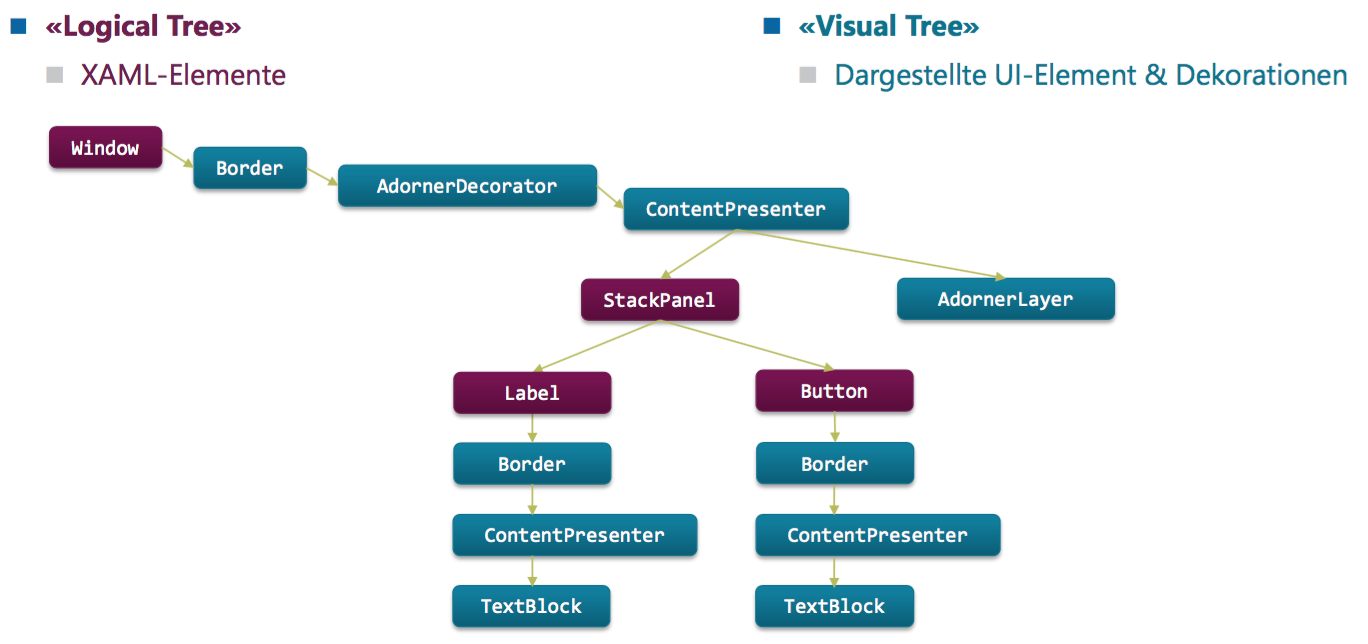
\includegraphics[scale=0.27]{LogicalVisual.png}
Der Logical-Tree entspricht der Strukutr der XAML-Elemente. Sie beschreibt die Beziehungen zwischen verschiedenen Elementen des UI. Es ist Zuständig für:
\begin{itemize}
    \item Dependency Properties erben
    \item Dynamische Ressourcen-Referenzen auflösen
    \item Elementnamen für Datenbindung nachschlagen
    \item Routed Events weiterleiten
\end{itemize}
Der Visual-Tree entspricht der grafischen Repräsentation und beinhaltet alle dargestellten Elemente gemäss der Vorlage jedes Controls. Es ist Zuständig für:
\begin{itemize}
    \item Visuelle Darstellung
    \item Vererben der Transparenzeinstellungen
    \item Vererben von Transformationen
    \item Vererben der IsEnabled-Property
    \item Hit-Testing
\end{itemize}
\paragraph{Property Syntax} XAML verwendet die Property Syntax wohingegen HTML beispielsweise Attribute Syntax verwendet.
\section{Layout und Controls}
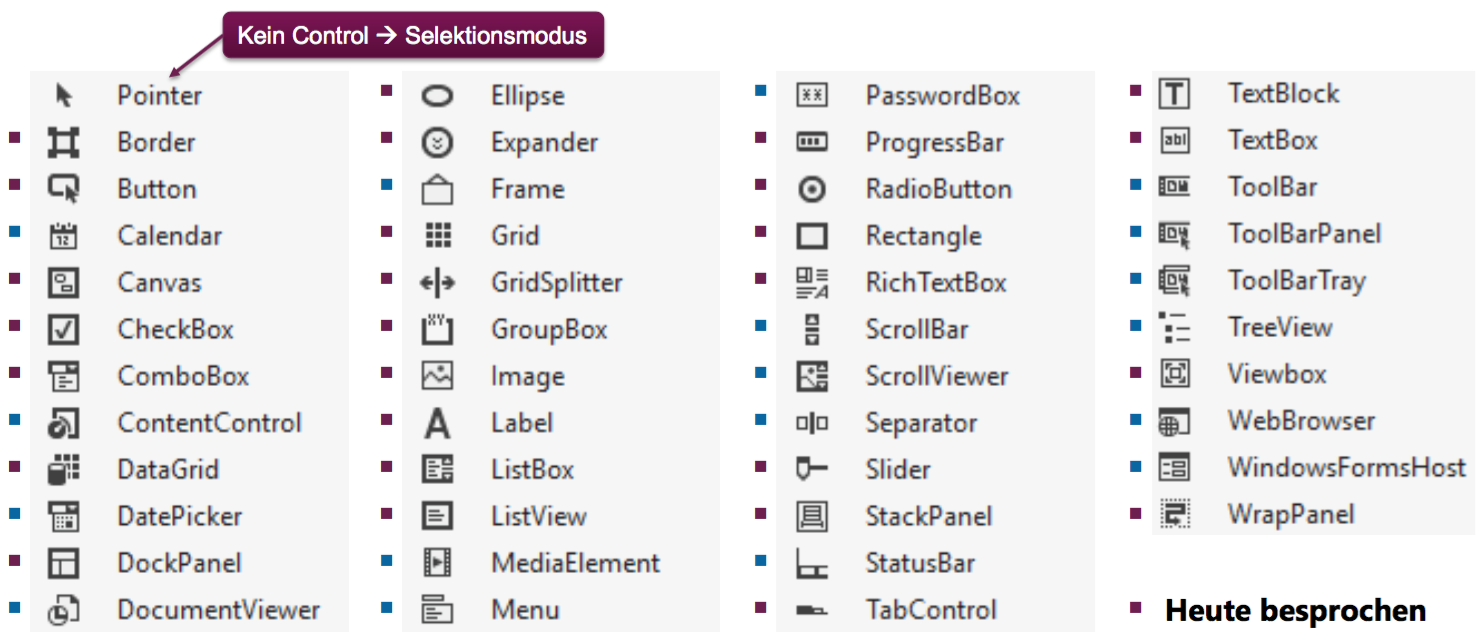
\includegraphics[scale=0.25]{ControlsOverview.png}
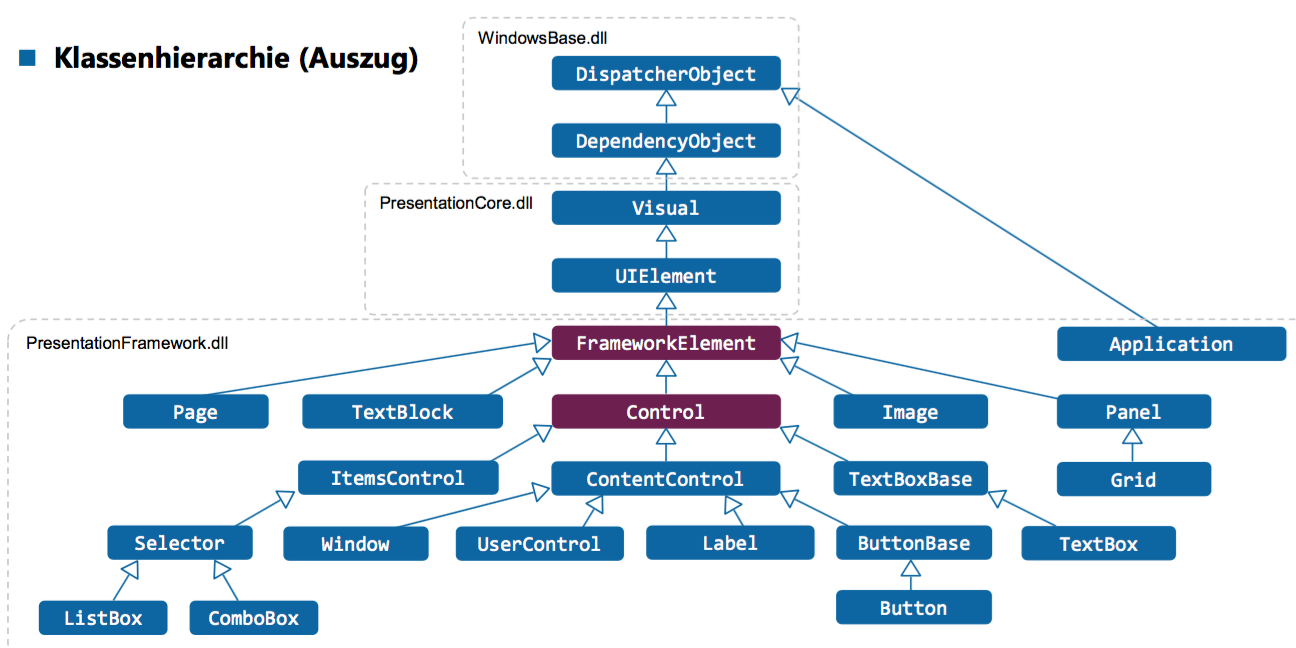
\includegraphics[scale=0.30]{Klassenhierarchie.png}
\paragraph{Grössenangaben} Zur Manipulation von Width und Height Attributen (\code{System.Windows.FrameworkElement}) kann man fixe Grössenangaben verwenden, diese werden als \code{double} Werte geschrieben. Wenn kein Kennzeichner angegeben ist (nur eine Zahl), wird automatisch \textit{Device Independent Pixel} verwendet $\left(\frac{1}{96}''\right)$. Qualfizierte Grössenangaben sind:
\begin{itemize}
\item \textbf{px} Device Independent Pixels $\left(1\text{px} = \frac{1}{96}''\right)$
\item \textbf{in} Inches (Zoll) $1\text{in} = 96\text{px}$
\item \textbf{cm} $1\text{cm} = \frac{96}{2.54}\text{px}$
\item \textbf{pt} Points $1\text{pt} = \frac{1}{72}'' = \frac{96}{72}\text{px}$
\end{itemize}
Zusätzlich kann man noch \code{MinWidth} und \code{MaxWidth} definieren. Bei Platzproblemen wird zuerst MinWidth, dann MaxWidth und dann Width evaluiert. Das Read-only Property \code{ActualWidth} kann verwendet werden um die Fenstergrösse während der Laufzeit abzufragen. 
\paragraph{Ausrichtung} HorizontalAlignment und VerticalAlignment Attribute manipulieren die Ausrichtung innerhalb des Containers. Es gibt auch HorizontalContentAlignment und VerticalContentAlignment für Inhaltsaurichtung beispielsweise für TextBox. Valide Werte sind: Left, Center, Right und Strecth für Horizontal bzw. Top, Center, Bottom und Stretch für Vertical. Strecth füllt jeweils die komplette Verfügbare Achse. 
\paragraph{Ränder \& Rahmen} Um Rahmengrössen anzupassen gibt es Margin, Padding, BorderThickness und CornerRadius. Für die ersten 3 sind folgende Werte zulässig
\begin{itemize}
\item \textbf{l,t,r,b}
\item \textbf{l,t} Left=Right, Top=Bottom
\item \textbf{x} Auf allen Seiten gleich viel Abstand
\end{itemize}
Bei Corner Radius gibt es nur eine zulässige Definition:
\begin{itemize}
\item TopLeft, TopRight, BottomRight, BottomLeft
\end{itemize}
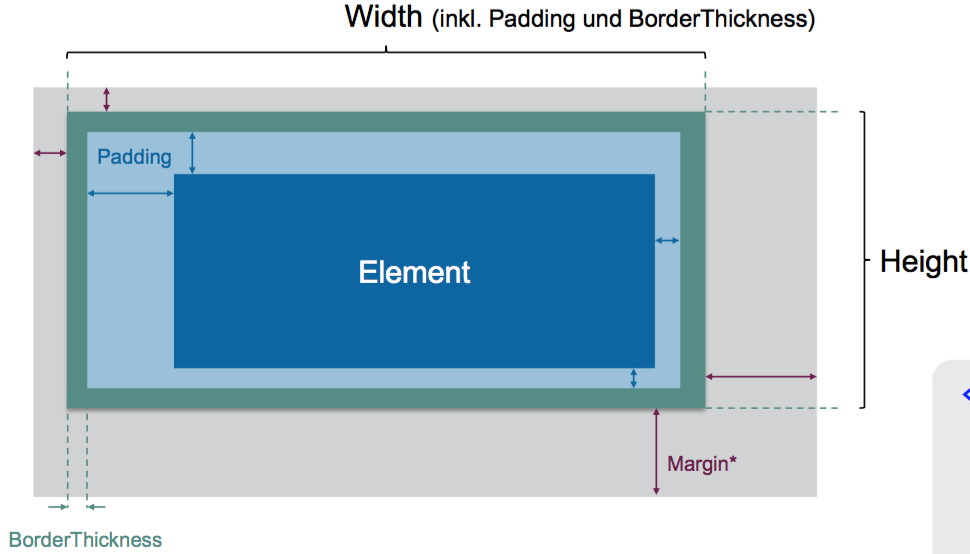
\includegraphics[scale=0.35]{Rahmen.png}
Auf jedes \textbf{UIElement} kann man noch \code{IsEnabled}, \code{SnapsToDevicePixels} (Rundet Pixelangaben auf physikalische Gerätepixelwerte) und \code{Visibility} (Collapsed, Hidden, Visible). Auf jedes \textbf{FrameworkElement} kann man \code{Name}, \code{Resource}, \code{Tag}, \code{Tooltip} und \code{UseLayoutRounding} anwenden. Auf jedes \textbf{Control} kann man \code{Background}, \code{BorderBrush}, \code{Foreground}, \code{FontFamily}, \code{FontSize}, \code{FontStrech}, \code{FontStyle} und \code{FontWeigt} anwenden.
\paragraph{Brush} Mit Brushes kann man einfache oder komplexe Farbverläufe darstellen. Es gibt 6 Pinseltypen
\begin{itemize}
\item SolidColorBrush (Einfarbig)
\item LinearGradientBrush (Einfacher Farbverlauf)
\item RadialGradient Farbverlauf (Runder Farbverlauf, errinert an Kugel)
\item ImageBrush (Bild innerhalb des Brushes)
\item DrawingBrush (Spezielle Muster)
\item VisualBrush (Komplexte Textdarstellung)
\end{itemize}
\paragraph{Clipping} Mit \code{ClipToBounds} kann man definieren, ob Child Controls an den Rändern des Parent Controls abgeschnitten werden sollen. Mit \code{Clip} kann man definieren welche Form zum Zuschneiden eines Controls verwendet werden soll.
\begin{lstlisting}[language=xml]
<Image.Clip>
    <EllipseGeometry
        RadiusX="100"
        RadiusY="75"
        Center="100, 75" />
</Image.Clip>
\end{lstlisting}
\subsection{Container Controls} Bei Container gibt es welche mit Layout und ohne Layout. Container mit Layout sind: \textbf{StackPanel}, \textbf{WrapPanel}, \textbf{DockPanel} und \textbf{Grid}. Container ohne Layout sind: \textbf{Canvas}, \textbf{ScrollViewer}, \textbf{Viewbox} und \textbf{Border}.
\paragraph{StackPanel}Das StackPanel und WrapPanel haben ein Attribut \code{Orientation} welches entweder auf \textit{Horizontal} oder \textit{Vertical} gesetzt werden kann. Die Elemente werden entsprechend Angeordnet
\paragraph{DockPanel}Das DockPanel ist ideal für eine Header, Footer Darstellung.
%TODO: W09-Layout und Controls, Folie 26, Dockpanel Grafik
Mit dem Attribut \code{DockPanel.Dock} kann man definieren, wo der Container sein wird. Beim DockPanel ist die Reihenfolge wichtig, denn der Verfügbare Platz wird in absteigender Reheinfolge verteilt
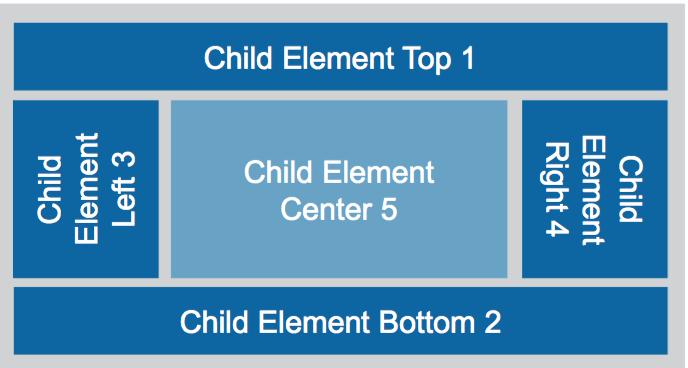
\includegraphics[scale=0.35]{DockPanel.png}
\paragraph{Grid} Im Grid können Child Elemente einer Zelle darin zugeordnet werden. Die Zeilen und Spalten müssen explizit angegeben werden
\begin{lstlisting}[language=xml, caption="3 x 3 Grid"]
<Grid>
    <Grid.ColumnDefinitions>
        <ColumnDefinition></ColumnDefinition>
        <ColumnDefinition></ColumnDefinition>
        <ColumnDefinition></ColumnDefinition>
    </Grid.ColumnDefinitions>
    <Grid.RowDefinitions>
        <RowDefinition></RowDefinition>
        <RowDefinition></RowDefinition>
        <RowDefinition></RowDefinition>
    </Grid.RowDefinitions>
</Grid>
\end{lstlisting}
Auf den einzelnen Definitions kann man \code{Width} und \code{Height} definieren (sowie Min/Max etc.). Ebenfalls ist es mit \code{RowSpan} bzw. \code{ColumnSpan} möglich, Elemente über mehrere Zellen/Spalten zu strecken. \\
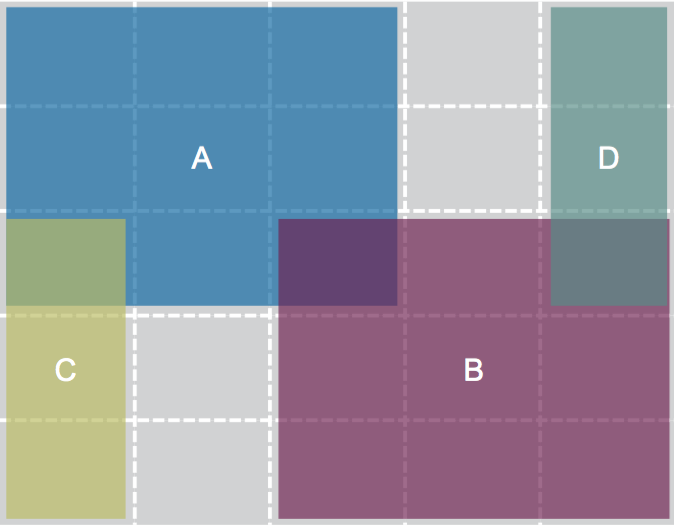
\includegraphics[scale=0.35]{Grid.png}
\begin{lstlisting}[language=xml]
<Grid>
    <Grid.ColumnDefinitions>...</Grid.ColumnDefinitions>
    <Grid.RowDefinitions>...</Grid.RowDefinitions>
    <Button Content="A"
        Grid.Column="0" Grid.Row="0"
        Grid.RowSpan="3" Grid.ColumnSpan="3" />
    <Button Content="B"
        Grid.Column="2" Grid.Row="2"
        Grid.RowSpan="3" Grid.ColumnSpan="3" />
    <Button Content="C"
        Grid.Column="0" Grid.Row="2"
        Grid.RowSpan="3" Grid.ColumnSpan="1" />
    <Button Content="D"
        Grid.Column="4" Grid.Row="0"
        Grid.RowSpan="3" Grid.ColumnSpan="1" />
</Grid>
\end{lstlisting}
\textbf{Spezialfall} Bei einem 1 x 1 Grid werden die Elemente in der Zelle gestapelt und man kann mit Alignments und Margin ein flexibles Layout erstellen. Mit dem GridSplitter kann man die Spalten und Zellengössen anpassen. Mit der SharedSizeGroup können mehrere Spalten/Zeilen verknüpft werden um eine einheitliche Breite/Höhe festzulegen.
\paragraph{Canvas} In einem Canvas Control haben alle Elemente eine absoulte Positionierung und es gibt keine Layout Logik. Die Position innerhalb des Canvas kann mittels Attached Properties festgelegt werden:
\begin{itemize}
\item \code{Canvas.Left}: Abstand vom linken Rand
\item \code{Canvas.Top}: Abstand vom oberen Rand
\item \code{Canvas.Right}: Abstand vom rechten Rand
\item \code{Canvas.Bottom}: Abstand zum unteren Rand
\item \code{Canvas.ZIndex}: Z-Position (Ebene) im Canvas
\end{itemize}
In Verbindung mit \code{Shapes} ist ein Canvas Control gut zum "{}programmierten Zeichnen"{} geeignet.
\begin{lstlisting}[language=xml]
<Canvas>
    <Rectangle
        Canvas.Left="80" Canvas.Top="60"
        Width="128" Height="80"
        Fill="#006aa6" />
    <Ellipse
        Canvas.Left="260" Canvas.Top="160"
        Width="120" Height="120"
        Fill="#6E1C50" />
    <Path
        Canvas.Left="120" Canvas.Top="64"
        Width="260" Height="200"
        Stroke="DarkGray" Stretch="Fill"
        Data="M1,0 L0,1"/>
</Canvas>
\end{lstlisting}
\paragraph{Shapes} Die Shapes Klasse beinhaltet \code{Ellipse}, \code{Polygon}, \code{Line}, \code{Polyline}, \code{Path} und \code{Rectangle}. Alle Shapes haben folgende Attribute:
\begin{itemize}
\item \textbf{Fill:} Brush für die Füllung
\item \textbf{Stroke:} Pen für Rahmen/Pinselstrich
\item \textbf{StrokeThickness:} Breite des Rahmens/Pinselstrichs
\item \textbf{StrokeDasharray:} Muster für gestrichelte Linien
    \subitem \textbf{"{}2 1"{}} ist das Verhätniss zwischen Linie/Lücke immer 2:1
    \subitem \textbf{"{}2 1 4 1"{}} ist das Verhältniss zuerst 2:1, dann 4:1 dann 2:1 etc.
\item \textbf{StrokeLineJoine:} Art des Übergangs bei Ecken
    \subitem \textbf{Miter:} Spitzer Rand
    \subitem \textbf{Bevel:} Abgeschnittener Rand
    \subitem  \textbf{Round:} Abgerundeter Rand
\end{itemize}
\paragraph{ViewBox} Skaliert, mittels Transformation, ein einzelnes Child Control um den Verfügbaren Platz auszunutzen. Das Attribut \code{Strech} kann verwendet werden um zu definieren wie das Control skaliert werden soll. Valid sind: \code{None} (keine Skalierung), \code{Uniform} (Vergrössern bis es ins Controll passt), \code{Fill} (Strecken, dass kompletter Platz verwendet wird), \code{UniformToFill} (Vergrössern und Strecken, dass Proportionen erhalten bleiben, aber ganzes Control ausgefüllt wird. Bei Übergrösse wird das Alignment berücksichtigt.
\paragraph{Border} Die Border zeichnet lediglich ein Rahmen um ein Child Control. Es kann mit Panels kombiniert werden.
\begin{lstlisting}[language=xml]
<Border Background="GhostWhite" CornerRadius="8,0,8,0"
        BorderBrush="#ddd" BorderThickness="1"
        Margin="10"
        Padding="10">
    <StackPanel Orientation="Vertical">
        <Button Margin="0,0,0,5" Content="Dock Sample 1" />
        <Button Margin="0,0,0,5" Content="Dock Sample 2" />
        <Button Margin="0,0,0,5" Content="Grid Sample 1" />
        <Button Margin="0,0,0,5" Content="Grid Sample 2" />
        <Button Margin="0,0,0,5" Content="Grid Sample 3" />
        <Button Margin="0,0,0,5" Content="Canvas Sample 3" />
    </StackPanel>
</Border>
\end{lstlisting}
\subsection{Input Controls}
\paragraph{Texteingabe} Für die Texteingabe gibt es die \code{TextBox} (Normalen Text Input, mit Option für mehrzeilige Eingabe), \code{RichTextBox} (Text Input mit Formatierung) und die \code{PasswordBox}.
\paragraph{Buttons} Es gibt verschiedene Arten von Buttons: \code{Button}, \code{RepeatButton} (Löst Click-Event wiederholt aus, bis Button losgelassen wird), \code{ToggleButton} (hat zwei Zustände), \code{RadioButton}, \code{CheckBox}.
\subsection{List Control}
\paragraph{Listen} Es gibt verschiedene Listen in WPF. Die \code{ListBox} ist eine komplett sichtbare (scrollable) Liste mit Daten. Diese Einträge können auch Formatierungen beinhalten.
\begin{lstlisting}
<ListBox SelectedIndex="1" SelectionMode="Multiple">
    <ListBoxItem>Erster Eintrag</ListBoxItem>
    <ListBoxItem>Zweiter Eintrag</ListBoxItem>
    <StackPanel Orientation="Horizontal">
        <Rectangle Width="10" Height="10" Fill="Blue" />
        <TextBlock Margin="10,0">Dritter Eintrag</TextBlock>
    </StackPanel>
</ListBox>
\end{lstlisting}
Die ComboBox ist eine normale DropDown Liste. Sie kann editierbar gemacht werden, mit \code{IsEditable} bzw. \code{IsReadOnly}.
\begin{lstlisting}[language=xml]
<ComboBox SelectedIndex="0">
    <ComboBoxItem>Erster Eintrag</ComboBoxItem>
    <ComboBoxItem>Zweiter Eintrag</ComboBoxItem>
</ComboBox>
\end{lstlisting}
Eine \code{ListView} ist ein Read-Only DataGrid, eine generalisierte Anzeige einer Liste (Explorer Ansichten).\\
Eine \code{TreeView} ist eine hierarchische Anzeige von Daten in einer Baumstruktur (Windows Explorer Pfad Baum).
\subsection{Beschriftungen} 
\paragraph{TextBlock} Dies ist eine einfache Textanzeige, kein vollwertiges Control. Es kann auch als einfaches "{}Spacer"{} Element gebraucht werden.
\paragraph{Label} Ein Label kann mittels Keyboard Shortcuts aufgerufen werden (vollwertiges Control). Es kann nicht nur Text anzeigen, sondern auch Layouts beinhalten und das Aussehen kann mittels Templates gestaltet werden.
\paragraph{ToolTip} Das ToolTip kann kontextbezongene Infos bei einem Mouse-Over anzeigen, es kann ebenfalls ein beliebiges Layout beinhalten. Bei deaktivierten Controls muss die Property \code{ToolTipService.ShowOnDisabled} gesetzt werden, wenn ToolTip trotzdem erscheinen soll.
%TODO: W09 - Layout und Controls, Folie 49, ToolTip Grafik
\begin{lstlisting}
<Button.ToolTip>
    <StackPanel>
        <TextBlock Text="Submit Button"
            FontWeight="Bold" />
        <TextBlock Text="Submits ..." />
    </StackPanel>
</Button.ToolTip>
\end{lstlisting}
\subsection{Wertebereiche}
\paragraph{Progress Bar} wird verwendet um den Benutzer auf eine lange andauernde Operation hinzuweisen. Mit Container Controls kann dieser beliebig dekoriert werden. 
\begin{lstlisting}[language=xml]
<ProgressBar Minimum="0" Maximum="100" Value="75" />
\end{lstlisting}
\paragraph{Slider} Der Slider gibt eine Auswahl aus einem vorgegeben Wertebereich zurück
\begin{lstlisting}[language=xml]
<Slider Maximum="100" Value="75" TickFrequency="10" TickPlacement="BottomRight" />
\end{lstlisting}
\subsection{Organisation}
\paragraph{GroupBox} gruppiert visuell zusammengehörende Controls
\begin{lstlisting}[language=xml]
<GroupBox Header="Mouse Handedness">
    <StackPanel>
        <RadioButton Content="Left-Handed" />
        <RadioButton Content="Right-Handed"
            IsChecked="True"/>
    </StackPanel>
</GroupBox>
\end{lstlisting}
\paragraph{Expander} ermöglicht das Ein und Ausblenden von Infos bei Bedarf. Er wird oft für Zusatzinformationen gebraucht.
\begin{lstlisting}[language=xml]
<Expander>
    <Expander.Header>More info</Expander.Header>
    <TextBlock TextWrapping="Wrap" Text="Drag ..." />
</Expander>
\end{lstlisting}
\paragraph{TabControl} teilt das UI in mehrere Seiten auf. Jedes \code{TabItem} enthält ein eigenes Layout. Das Header Attribut kann mit beliebigem Layout gefüllt werden.
\begin{lstlisting}[language=xml]
<TabControl>
    <TabItem Header="1 - Intro">
        <Grid Margin="10">
        ...
        </Grid>
    </TabItem>
    <TabItem Header="2 - Daten" />
    <TabItem Header="3 - Optionen" />
    <TabItem>
        <TabItem.Header>
            <StackPanel Orientation="Horizontal">
                <Grid>
                    <Ellipse Fill="Silver" Width="16"
                        Height="16" />
                    <Label Content="4" FontSize="10"
                        Foreground="White" />
                </Grid>
            <TextBlock Text="Review" />
            </StackPanel>
        </TabItem.Header>
    </TabItem>
</TabControl>
\end{lstlisting}
\paragraph{Eigene Controls} Es gibt zwei Arten von Controls. Das \code{UserControl} welches als \textbf{Komposition} implementiert wird. Es ist eine Wiederverwendbare Zusammenstellung mehrer COntrols als Gruppe und besteht aus einem XAML und Code-Behind. Es kann nicht mit Styles/Templates umgehen.\\
Das \code{CustomControl} ist eine Ableitung der zu verändernden Klasse. Es erweitert ein bestehendes Control um neue Funktionen. Es besteht aus einem Code-File und ggf. aus einem Standart-Style. Es kann mit Styles/Templates umgehen.
\section{Menüs}
\subsection{Benutzerführung}
Die höchste Klasse jeder XAML App ist die \code{System.Windows.Application}. Diese beinhaltet u.a. ein \code{Current} Property (Singelton) welches statischen Zugriff auf das Application Objekt bietet, das \code{MainWindow}, das Zugriff auf das Hauptfenster bietet und den \code{ShutdownMode} welche das Verhalten beim Programmende definiert.
\paragraph{Current} Das Application Objekt ist als Singelton implentieret. Um es innerhalb der App zu verwenden, muss es oft gecastet werden.
\begin{lstlisting}
public App MyApp => Application.Current as App;
\end{lstlisting}
\paragraph{ShutdownMode} Der ShutdownMode definiert das Verhalten der App beim beenden, davon gibt es 3.
\begin{itemize}
\item \code{OnLastWindowClose}: Dies ist das Standardverhalten, die App beendet sich, sobald das letzte Fenster geschlossen wurde
\item \code{OnMainWindowClose}: Die App wird beendet sobald das Hauptfenster geschlossen wird
\item \code{OnExplicitShutdown}: Die App wird erst beendet, wenn die \code{Shutdown()} Methode aufgerufen wurde.
\end{itemize}
\paragraph{StartupUri} Dies ist der Name der UI Ressource, die beim Start angezeigt werden soll, es ist normalerweise ein \verb+Window+
\paragraph{Windows} Das \code{Windows} Property ist eine Liste aller instanziierter Fenster (Window-Objekte) innerhalb der App.
\paragraph{Application-Klasse Methoden} Die \verb+LoadComponent+ Methode lädt eine XAML-Ressource.
\begin{lstlisting}
public static object LoadComponent(Uri uri)
\end{lstlisting}
Der Rückgabetyp muss in den korrekten Typ gecastet werden.\\
Die \verb+FindResouce+ Methode, sucht eine Ressource mit dem angegeben Namen. Es durchsucht App-Ressourcen und System-Ressourcen. Der Rückgabetyp muss ebenfalls in den korrekten Typ gecastet werden.
\begin{lstlisting}
public object FindResource(object resourceKey)
\end{lstlisting}
Die \verb+Shutdown+ Methode beendet die App und gibt optional einen mitgegebenen Exit Code ans System zurück.
\begin{lstlisting}
public void Shutdown([int exitCode])
\end{lstlisting}
\paragraph{Application-Klasse Events}
\begin{itemize}
\item \verb+Activated+: Die App wurde aktivitert (in den Vordergrund geholt)
\item \verb+Deactivated+: Die App wurde deaktiviert
\item \verb+DispatcherUnhandledException+: Eine nicht gefangene Exception ist aufgetreten
\item \verb+Exit+: Die App wird gleich beendet
\item \verb+FragmentNavitation+: Es wurde zu einem bestimmten \verb+NavigationWindow+/\verb+Frame+ navigiert
\item \verb+LoadCompleted+: Aktuelles \verb+NavigationWindow+/\verb+Frame+ wurde vollständig geladen
\item \verb+Navigated+: Aktuelles \verb+NavigationWindow+/\verb+Frame+ wurde gefunden
\item \verb+Navigating+: Navigation zu einem \verb+NavigationWindow+/\verb+Frame+  wurde angefordert
\item \verb+NavigationFailed+: Navigation zu einem \verb+NavigationWindow+/\verb+Frame+ ist fehlgeschlagen
\item \verb+NavigationProgress+: Statusinformation zum Downloadstatus bei Internet-Ressourcen
\item \verb+NavigationStopped+: Ladevorgang des Inhalts der \verb+NavigationWindow+/\verb+Frame+ wurde gestoppt
\item \verb+SessionEnding+: Windows Session wird beendet
\item \verb+Startup+: Die App startet gerade
\end{itemize}
\paragraph{SplashScreen} Es gibt 2 Arten einen SplashScreen zu implementieren. Die automatische Variante ist, ein Bild in das Projekt zu kopieren und bei den FileProperties \verb+BuildAction+ auf SplashScreen zu setzten. Die kontrollierte Variante ist, in der \verb+App_OnStartup+ Methode den SplashScreen zu instanzieren und anzuzeigen.
\begin{lstlisting}
private void App_OnStartup(object sender, StartupEventArgs e)
{
    var screen = new SplashScreen("media/splash.png");
    screen.Show(true);
}
\end{lstlisting}
Der Screen muss dann natürlich auch irgendwann wieder ausgeblendet werden. Alternativ kann man diesen auch nach einer gewissen Zeit ausblenden.
\begin{lstlisting}
private void App_OnStartup(object sender, StartupEventArgs e)
{
    var screen = new SplashScreen("media/splash.png");
    screen.Show(true); // in den Folien steht false
    Thread.Sleep(2000);
    screen.Close(TimeSPan.FromMilliseconds(500));
}
\end{lstlisting}
\subsection{Window Klasse}
Die \verb+Window+ Klasse beschreibt ein Fenster. Sie ist abgeleitet von \verb+ContentControl+ und erlaubt genau 1 Child Element (\verb+LayoutContainer+).
\begin{itemize}
\item \verb+Icon+: Dieses Property beinhaltet eine ICO-Datei, die als Fenster Icon verwendet wird (Ausführbaren Datei und Fensterttitel)
\item \verb+ShowInTaskBar+: Ein Property das angibt, ob das Fenster in der Taskleite angezeigt wird
\item \verb+Topmost+: Zeigt Fenster über allen andern Fenstern der Anwendung an
\item \verb+SizeToContent+: Legt fest, ob die Grösse eines Fensters automatisch an die Grösse des Inhalts angepasst wird.
    \subitem \verb+Manual+: Fenstergrösse anhand Width/Height Angabe(Standart)
    \subitem \verb+Height+: Höhe wird automatisch anhand des Inhalts festgelegt
    \subitem \verb+Width+: Breite wird automatisch anhand des Inhalts festgelegt
    \subitem \verb+WidthAndHeight+: Breite und Höhe werden automatisch anhand des Inhalts festgelegt
\item \verb+ResizeMode+: Gibt an, wie sich die Fenstergrösse ändern darf. Je nach Einstellung werden zusätzlich die Schaltflächen Minimieren/Maximieren im Fenstertitel angezeigt
    \subitem \verb+NoResize+: Fenstergrösse nicht änderbar
    \subitem \verb+CanMinimize+: Fenster kann minimiert und wiederhergestellt werden
    \subitem \verb+CanResize+: Fenstergrösse kann frei verändert werden (Standard)
    \subitem \verb+CanResizeWithGrip+: Wie \verb+CanResize+ aber mit zusätzlichem Resize Grip unten rechts im Fenster
\item \verb+WindowsStartupLocation+: Legt die Postition beim Start fest
    \subitem \verb+CenterOwner+: Fenster wird in Mitte des aufrufenden angezeigt
    \subitem \verb+CenterScreen+: Fenster wird in der Mitte des Bildschirm angezeigt
    \subitem \verb+Manual+: Position wird durch Left/Top Angabe bestimmt (Standart)
\item \verb+WindowState+: Beschreibt die Fensterzustände (Normal, Minimized, Maximized)
\item \verb+WindowStyle+: Gibt den Rahmentyp des Fensters an:
    \subitem \verb+None+: Nur das Client Area ist sichtbar
    \subitem \verb+SingleBorderWindow+: Fenster mit einfachem (dünnem) Rahmen
    \subitem \verb+ThreeDBorderWindow+: Fenster mit 3D Rahmen
    \subitem \verb+ToolWindow+: Verankertes Tool-Fenster
\end{itemize}
\paragraph{Window-Klasse Methoden}
\begin{itemize}
\item \verb+Activate+: Fenster aktivieren
\item \verb+Close+: Fenster schliessen
\item \verb+DragMove+: Ermöglich das Verschieben des Fensters, falls die linke Maustaste gedrückt ist
\item \verb+GetWindow+: Statische Methode, ruft das Root-Window Objekt zum Control ab (DI)
\item \verb+Hide+: Macht das Fenster unsichtbar
\item \verb+Show+: Zeigt das Fenster an
\item \verb+ShowDialog+: Zeigt das Fenster an und blockiert, bis das Fenster geschlossen wird
\end{itemize}
\paragraph{Window-Klasse Events}
\begin{itemize}
\item \verb+Activated+: Fenster wurde aktiviert
\item \verb+Closed+: Fenster wurde geschlossen
\item \verb+Closing+: Fenster wird gleich geschlossen
\item \verb+ContentRendered+: Fensterinhalt wurde gezeichnet
\item \verb+Deactivated+: Fenster wurde deaktiviert
\item \verb+LocationChanged+: Position des Fensters wurde geändert
\item \verb+StateChanged+: WindowState hat geändert
\end{itemize}
\subsection{Dialogfenster} 
Dialogfenster dienen zum Abruf von Daten und sind meist Modal (blockierend). \\
Ein Dialogfenster wird mit der Methode \verb+ShowDialog+ angezeigt. Im Dialogfenster kann die Property DialogResult gesetzt werden (boolean). Sobald dies gesetzt wurde wird das Dialogfenster geschlossen. 
\begin{lstlisting}[language=xml]
<Button Content="Cancel" IsCancel="true" />
<Button Name="OkButton" Content="OK" IsDefault="true" Click="OkButton_OnClick" />
\end{lstlisting}
Das \verb+IsCancel+ Property schliesst bei \verb+true+ das Dialogfenster automatisch (kein Event-Handling).
\begin{lstlisting}
private void OkButton_OnClick(object sender, ReoutedEventargs e)
{
    SelectedCustomer = "MaxMuster";
    // trigger dialog close as side effect
    DialogResult = true; 
}
\end{lstlisting}
\paragraph{Fenster mit Spezialformen} Die Fensterrahmen können mittels Clipping verändert werden. Das setzt jedoch folgende Fenstereigenschaften voraus:
\begin{itemize}
\item \verb+AllowsTransparency=true+
\item \verb+WindowStyle=none+
\item \verb+ResizeMode=NoResize+
\end{itemize}
Man kann die Form in \verb+Window.Clip+ mittels einem Geometry-Element festlegen
\begin{lstlisting}[language=xml]
<!-- Rechteck mit abgerundeten Raendern -->
<Window.Clip>
    <RectangleGeometry RadiusX="8" RadiusY="8" Rect="0,0,800,600" />
</Window.Clip>
\end{lstlisting}
\subsection{Menu}
Die Menüs sind herkömmliche Windows-Menüs und werden üblicherweise am oberen Fensterrand angedockt. Mit dem Property \verb+IsMainMenu=true+ kann man das Menü standartmässig als Hauptmenü definieren.
\paragraph{MenuItem} MenuItems sind beliebig verschachtelbar. Sie haben ein \verb+Header+ als anzuzeigenden Texts (Underscore = Accelerator-Key), \verb+IsCheckable+ definiert, ob der Eintrag ein Zustand ist (mit \verb+IsChecked+ kann Zustand gesetzt bzw. geprüft werden). Das \verb+InputGestureText+ Property definiert, definiert einen Text, der im MenuItem rechtsbündig angezeigt wird (Shortcuts wie Ctrl+V), um zu Funktionieren müssen diese noch behandelt werden, beispielsweise mit Commands.
\begin{lstlisting}[language=xml]
<Menu DockPanel.Dock="Top">
    <MenuItem Header="_File">
        <MenuItem Header="_Recent">
            <MenuItem Header="Secret.txt" />
            <MenuItem Header="TopSecret.txt" />
        </MenuItem>
        <Separator />
        <MenuItem Header="E_xit" InputGestureText="CTRL + Q" />
    </MenuItem>
    <MenuItem Header="_Edit">
        <MenuItem Header="_Cut" InputGestureText="CTRL + X" />
        <MenuItem Header="C_opy" InputGestureText="CTRL + C" />
        <MenuItem Header="_Paste" InputGestureText="CTRL + V" />
        <Separator />
        <MenuItem Header="_Settings">
            <MenuItem Header="_Always On Top" IsChecked="True"></MenuItem>
            <MenuItem Header="_Modern UI" IsChecked="false"></MenuItem>
        </MenuItem>
    </MenuItem>
</Menu>
\end{lstlisting}
\paragraph{Kontextmenus} Das \verb+ContextMenu+ stellt ein kontextspezifisches Menü zur verfügung. Es funktioniert wie das Menü und kann direkt mit der Property-Syntax für ein Control erstellt werden.
\begin{lstlisting}[language=xml]
<Button.ContextMenu>
    <ContextMenu>
        <MenuItem Header="Hilfe" />
        <MenuItem Header="Fehler melden" />
    </ContextMenu>
</Button.ContextMenu>
\end{lstlisting}
\paragraph{StatusBar} Die Statusbar dient zur Anzeige von zusätzlichen Informationen (meist am unteren Fensterrand). Es ist ein Container, ähnlich wie beim DockPanel, dabei füllt das letzte Element die ganze restliche Breite.
\begin{lstlisting}[language=xml]
<StatusBar DockPanel.Dock="Bottom">
    <StatusBarItem Width="150">Press CTRL + Q to quit</StatusBarItem>
    <Separator />
    <StatusBarItem>Ready</StatusBarItem>
</StatusBar>
\end{lstlisting}
Für Kontextbezogene Statusinformationen können \verb+StatusBarItem+ Elemente benannt werden und dann programmatisch darauf zugegriffen werden, oder man arbeitet mit Databinding.
\paragraph{Toolbar} kann entweder ein \verb+ToolBarTray+ sein, der als Container für Toolbars dient, oder ein \verb+Toolbar+ der als Container für Toolbar-Buttons und sonstige Toolbar-Controls dient. Die ToolBarTray ermöglicht das Verschieben und Umgruppieren der Toolbars und ist typischerweise angedockt. \\
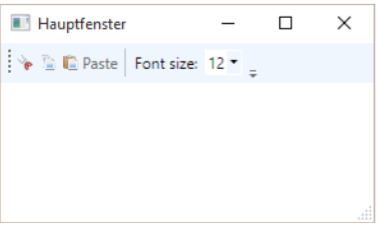
\includegraphics[scale=0.40]{Toolbar.png}
\begin{lstlisting}[language=xml]
<ToolBarTray DockPanel.Dock="Top">
    <ToolBar>
        <Button Command="Cut" ToolTip="...">
            <Image Source="/media/clip_cut.png" Width="12" Height="12" />
        </Button>
    <Button Command="Copy" ToolTip="Copy selection to Windows Clipboard.">
        <Image Source="/media/clip_copy.png" Width="12" Height="12" />
    </Button>
    <Button Command="Paste" ToolTip="Paste from Windows Clipboard.">
        <StackPanel Orientation="Horizontal">
            <Image Source="/media/clip_paste.png" Width="12" Height="12" />
            <TextBlock Margin="3,0,0,0">Paste</TextBlock>
        </StackPanel>
    </Button>
    <Separator />
    <Label>Font size:</Label>
    <ComboBox>
        <ComboBoxItem>10</ComboBoxItem>
        <ComboBoxItem IsSelected="True">12</ComboBoxItem>
        <ComboBoxItem>14</ComboBoxItem>
        <ComboBoxItem>16</ComboBoxItem>
    </ComboBox>
    </ToolBar>
</ToolBarTray>
\end{lstlisting}
\paragraph{Ribbon} Das Ribbon ist seit Office 2007 bekannt und ist seither immer stärker verbreitet. 
\begin{lstlisting}[language=xml]
<Ribbon Name="Ribbon">
    <Ribbon.ApplicationMenu>
        <RibbonApplicationMenu SmallImageSource="media/home.png">
            <RibbonApplicationMenuItem Header="Hello _Ribbon"
                Name="MenuItem1"
                ImageSource="media/home.png"/>
        </RibbonApplicationMenu>
    </Ribbon.ApplicationMenu>
    <RibbonTab x:Name="HomeTab" Header="Start">
        <RibbonGroup x:Name="Clipboard" Header="Clipboard">
            <RibbonButton x:Name="Button1" Label="Paste"
                LargeImageSource="media/clip_paste.png" />
            <RibbonButton x:Name="Button2" Label="Cut"
                SmallImageSource="media/clip_cut.png" />
            <RibbonButton x:Name="Button3" Label="Copy"
                SmallImageSource="media/clip_copy.png" />
        </RibbonGroup>
    </RibbonTab>
</Ribbon>
\end{lstlisting}
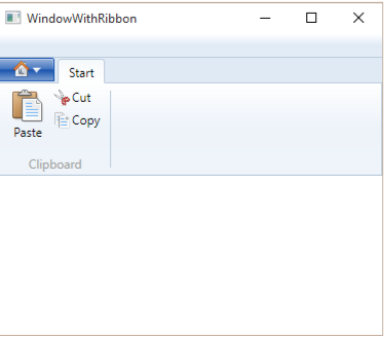
\includegraphics[scale=0.35]{Ribbon.png}
\section{Commands} bieten eine Alternative zum Event. Commands müssen nicht abgefangen und behandelt werden, sie werden durch die Control selbst aufgerufen. Es ist eine standartisierte Ausführung eines Befehls und ermöglicht die Wiederverwendung derselben Aktion. Eine Command-Methode muss \verb+RoutedUICommand+ als Rückgabetyp haben und statisch sein.
\begin{lstlisting}
public static RoutedUICommand MyCutCommand = new RoutedUICommand(
    "Ausschneiden",
    "MyCut",
    typeOf(WindowWithToolbar)
);
\end{lstlisting}
Der \verb+RoutedUICommand+ nimmt auch noch einen 4. Paramter entgegen, in dem man \verb+InputGestures+ entweder einzeln oder als \verb+InputGestureCollection+ mitgeben kann.
\begin{lstlisting}[language=xml]
<MenuItem Header="_Cut" InputGestureText="CTRL + X" Command="local:WindowWithToolbar.MyCutCommand" />
\end{lstlisting}
Commands können auch an Event-Handler gebunden werden und Shortcuts definiert werden.
\begin{lstlisting}[language=xml]
<!-- Binding an Event -->
<Window.CommandBindings>
    <CommandBinding Command="local:WindowWithToolbar.MyCutCommand" Executed="MyCutCommand_Executed" />
</Window.CommandBindings>
<!-- Shortcut definieren -->
<Window.InputBindings>
    <KeyBinding Key="X" Modifiers="Control" Command="local:WindowWithToolbar.MyCutCommand" />
</Window.InputBindings>
\end{lstlisting}
Im Code-Behind kann dann wie gewohnt ein Handler definiert werden.
\begin{lstlisting}
public void MyCutCommand_Executed(object sender, ExecutedRoutedEventArgs e){ ... }
\end{lstlisting}
\section{Automated UI Testing}
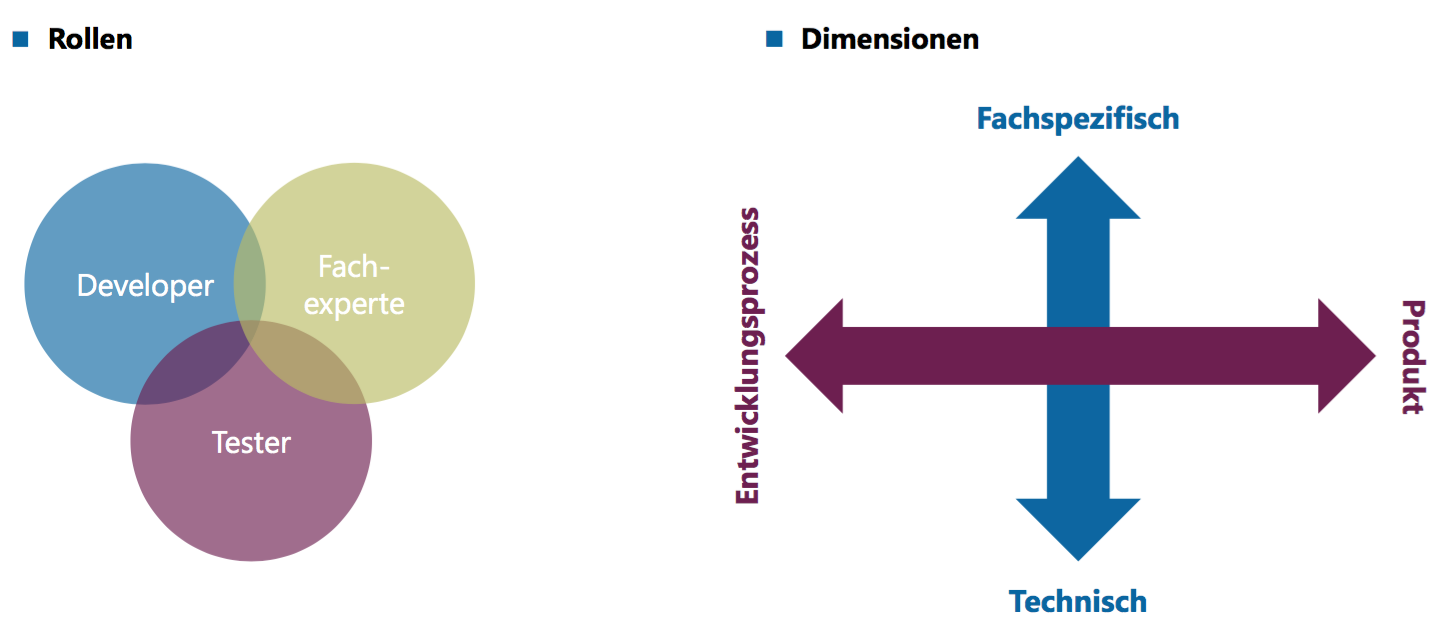
\includegraphics[scale=0.25]{Testing1.png}
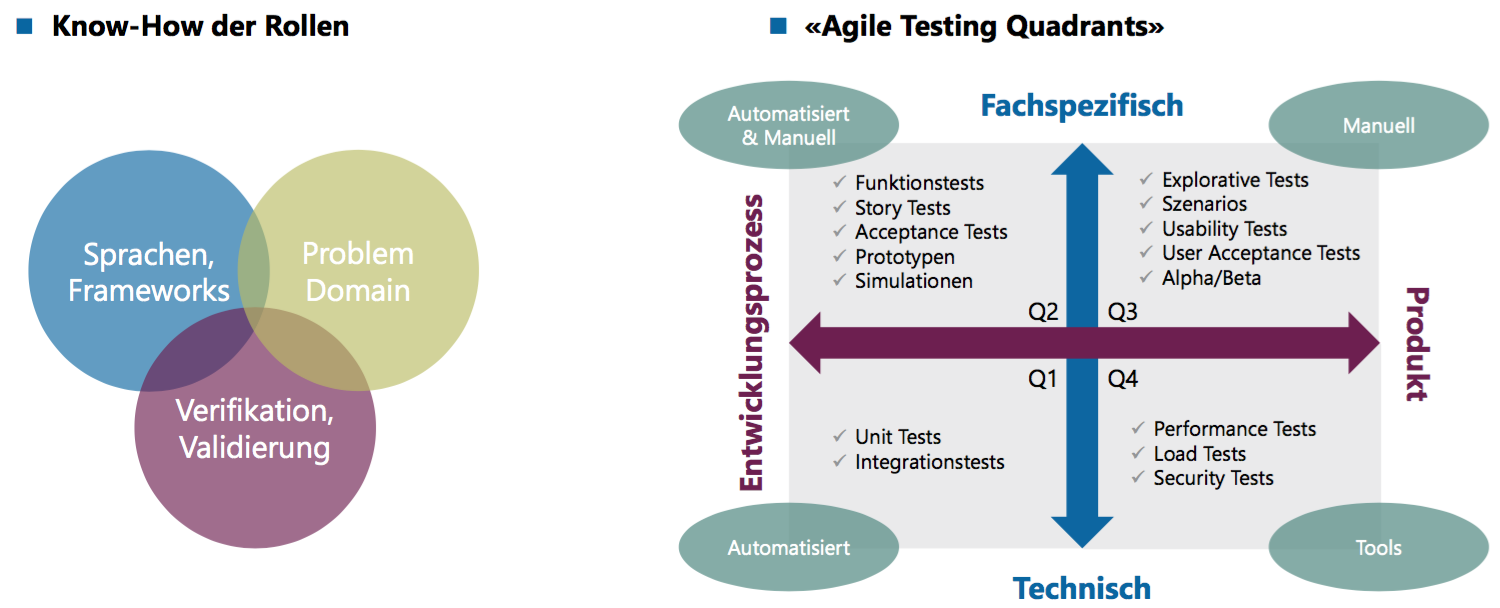
\includegraphics[scale=0.25]{Testing2.png}
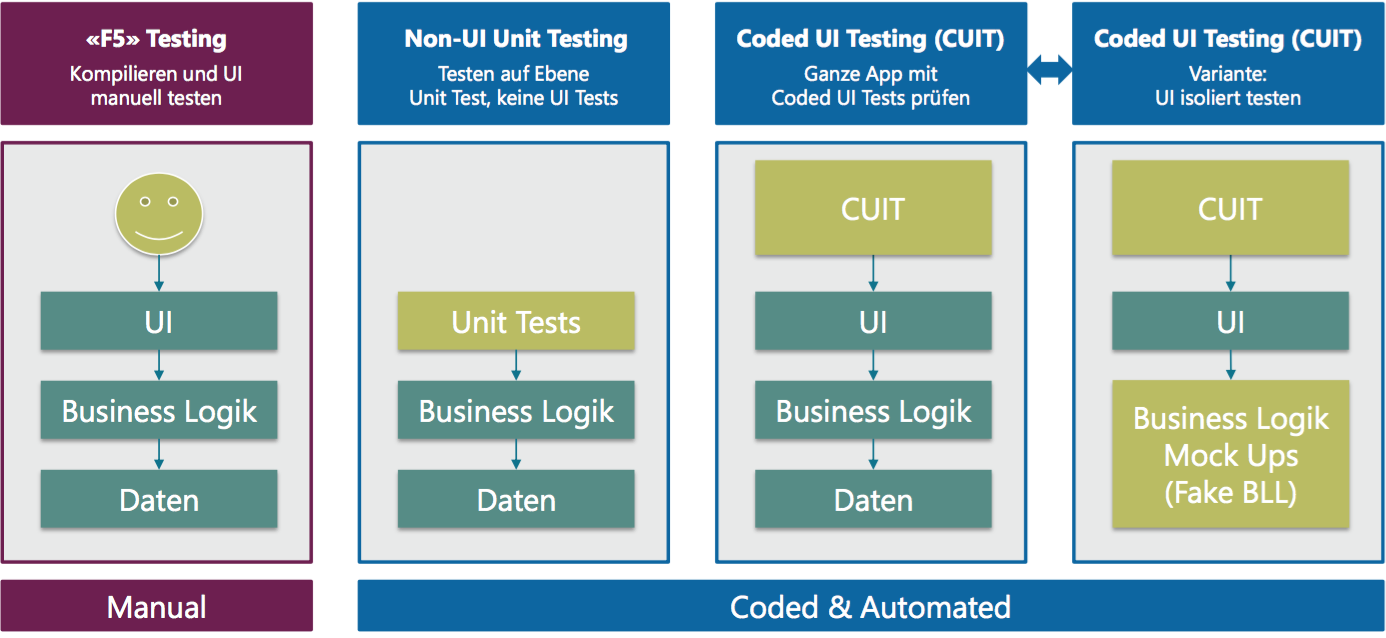
\includegraphics[scale=0.25]{Testing3.png} \\
Es gibt 4 Varianten UIs zu testen. Das \textbf{Non-UI Unit Testing} Test auf Code Ebene (normale Unit-Tests) und führt keine UI-Tests durch. Das \textbf{Coded UI Testing (CUIT)} testet die ganze App mit Coded UI Tests. Diese Variante kann man auch mit isolierten UI Komponenten durchführen, welche dann aber Fake Komponenten benötigen (die 4. Variante ist das F5-Testing, der Benutzer testet die App gleich selbst).
\subsection{TestStack}
Der TestStack ist eine Sammlung von OpenSource Projekten um Tests in .NET Projekten zu automatisieren. Dazu gehört das \textbf{TestStack.White} Framework. Es ist ein CUIT-FW für WPF und basiert auf Microsofts UI Automation Framework. \\
Als Vorbereitung muss man eine Testklasse erstellen.
\begin{lstlisting}
[TestClass]
public class MyUiTest
{
    [TestMethod]
    public void MyUiTestMethod(){ ... }
}
\end{lstlisting}
Danach muss man das Verzeichnis mit der WPF App Assembly festlegen. Dies kann dann als Read-Only Property in der Testklasse hinzugefügt werden.
\begin{lstlisting}
// Directory in which tests are running
public string BaseDir => Path.GetDirectoryName(Assembly.GetExecutingAssembly().Location);
// System under test
public string SutPath => Path.Combine(BaseDir, ${nameof(MenusAndCommands)}.exe);
//$
\end{lstlisting}
Nun kann man die Tests entwickeln. \\
Zuerst neues Application Objekt aus dem WPF App Assembly erstellen:
\begin{lstlisting}[caption="Neues Application Objekt aus dem WPF App Assembly erstellen"]
var app = Application.Launch(SutPath);
\end{lstlisting}
Die Variable enthät ein UI-Automatisierungsobjekt des Typs \verb+TestStack.Whie.Application+.
Danach kann man die Fenster abrufen:
\begin{lstlisting}
// Mit Fenstertitel abrufen
var window = app.GetWindow("Hauptfenster", InitializeOption.NoCache);
// Aus Liste der Fenster abrufen
var window = app.GetWindows.First();
// Anhand der ID(Name-Attribut) abrufen
var window = app.getWindow(SearchCriteria.ByAutomationId"(Win1"), InitializeOption.NoCache);
\end{lstlisting}
Die Variable \verb+window+ enthäht nun ein UI-Automatisierungsobjekt des Typs \verb+TestStack.White.UIItems.WindoItems.Window+.\\
Danach muss man die Controls abrufen:
\begin{lstlisting}
// Anhand Beschriftung abrufen
var button = window.Get<Button>(SearchCriteria.ByText("Speichern"));
// Anhand ID(Name-Attribut) abrufen
var button window.Get<Button>("SaveButton");
\end{lstlisting}
Die Variable \verb+button+ enthält nun ein UI-Automatisierungsobjekt des Typs \verb+TestStack.White.UIItems.Button+.\\
Schlussendlich können Aktionen ausgeführt werden:
\begin{lstlisting}
Assert.AreEqual("Speichern", button.Text);
button.Click();
Assert.AreEqual("Gespeichert!", button.Text);
\end{lstlisting}
\begin{lstlisting}
var input = window.Get<TextBox>("NameInput");
Assert.IsTrue(string.IsNullOrEmpty(input.Text));
var newText = "You've been hacked!";
input.Text = newText;
Assert.AreEqual(newText, input.Text);
\end{lstlisting}
Schlussendlich muss die App noch mittels \verb+app.Close()+ beendet werden.\\
Mit \verb+Desktop.CaptureScreenshot()+ erhält man ein Bitmap Objekt mit einem Bild des aktuellen Bildschirms.
\begin{lstlisting}
var screenshot = Desktop.CaptureScreenshot();
var path = System.IO.Path.Combine(BaseDir, "screenshot.png");
screenshot.Save(path, ImageFormant.Png);
\end{lstlisting}


\section{GUI Design}
\subsection{WPF Ressourcen}
Mit WPF Ressourcen kann man nützliche Objekte (Brushes, Styles, Templates etc.) zentral definieren und wiederverwenden.
\subsection{Resources}
\paragraph{Physikalische Ressourcen} In den File Properties kann man eine Datei als WPF-Ressource deklarieren welche dann in die Binärdatei einkompiliert werden. Zugegriffen kann dann mittels Resource-Key (relativer Pfadname).
\paragraph{Resource} Jedes beliebige Objekt in XAML kann als Ressource definiert werden. Es bird mit einem Key-Attribut und dem x-Namespace benannt.
\begin{lstlisting}[language=xml]
<Application.Resources>
    <SolidColorBrush x:Key ="MyButtonBackground" Color="#EEEEEE" />
</Application.Resources>
\end{lstlisting}
Unter diesem Key sind Ressourcen dann auch ansprechbar
\begin{lstlisting}[language=xml]
<Button Background="{StaticResource MyButtonBackground}" Content="Save" />
\end{lstlisting}
\paragraph{ResourceDictionary} Ist ein Behälter um Ressourcen zu speichern. Es indexiert nach dem Ressourcen-Namen (\verb+x:Key+) und kann in allen Elementen, welche von FrameworkElement ableiten, verwendet werden. Wenn auf eine Ressource zugegriffen werden möchte, wird \begin{enumerate*}[label=\itshape \arabic*\upshape.]\item Key im Element und allen Parent-Nodes gesucht (Logical Tree), \item dann wird der Key in \verb+Application.Resources+ gesucht, \item als letztes wird in System-Ressourcen gesucht.\end{enumerate*}. Die Reheinfolge im XAML-Code ist wichtig.
\paragraph{System Ressources} Auf Ressourcen in Namespace \verb+System.Windows+ kann man mittels statischer Properties zugegriffen werden. Dazu gehören: \verb+SystemColors+, \verb+SystemFonts+ und \verb+SystemParamters+.
\begin{lstlisting}[language=xml]
StaticResource="{StaticResource[name]}"
\end{lstlisting}
Die Statische Bindung macht CompileTime Check und findet Fehler früh.
\begin{lstlisting}[language=xml]
DynamicResource="{DynamicResource[name]}"
\end{lstlisting}
Anstelle von \verb+[name]+ steht der Key der Ressource
In der Dynamische Bindung wird ein RuntimeCheck gemacht und lässt dynamisch erzeugte und geladene Ressourcen zu. Beim Static Binding wird bei Objektkonstruktion ausgewertet, beim Dynamic Binding einmal pro Zugriff.
\paragraph{FindResource} Mit der Methode \verb+FrameworkElement.FindResources+  können Zugriffe auf XAML Resourcen gemacht werden.
\begin{lstlisting}
var okText = (string)FindResource("OkText");
var bgBrush = FindResource("DarkBrush") as Brush;
\end{lstlisting}
\section{Umgang mit Daten}
Ein grosses Feature von WPF ist das DataBinding. 
\paragraph{Markup Extensions}
\begin{itemize}
\item \verb+{x:Type [Datentyp]}+: Liefert angegebene Klasse
\item \verb+{x:Static [Pfade]}+: Bindet eine Konstante, statische Property, Feld oder Enum
\item \verb+{x:Null}+: Null Wert
\item \verb+{StaticResource [Name]}+: Statische Bindung an Ressource
\item \verb+{DynamicResource [Name]}+: Dynamische Bindung an Ressource
\item \verb+{Binding ...}+: Data Binding Ausdruck
\item \verb+{RelativeSource ... }+: Setzt die Data Binding Source auf eine relevanten Bezug im Logical Tree
\item \verb+{TemplateBinding ...}+: Bindet Wert an Eigenschaft des mittels Template dargestellten Controls
\item \verb+{x:Reference ...}+: Abk. für \verb+{Binding Elementname=...}+
\end{itemize}
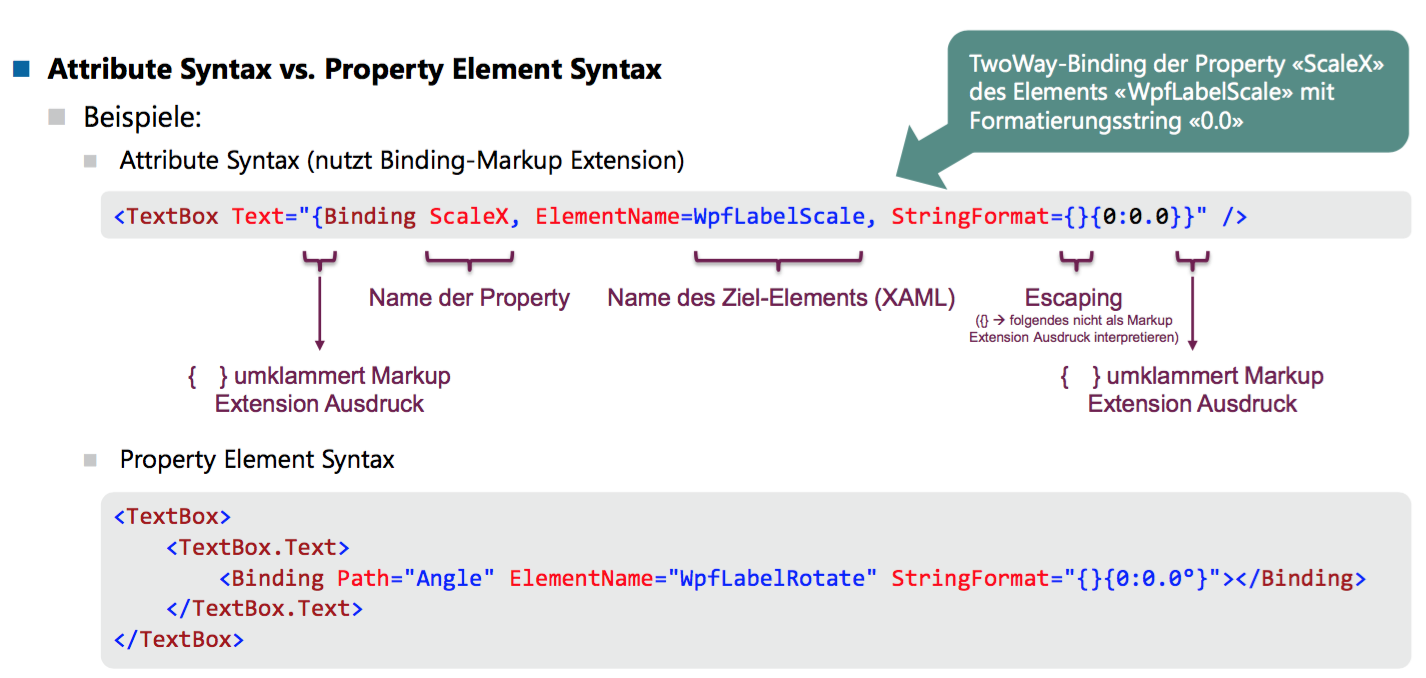
\includegraphics[scale=0.25]{DataBinding.png}
\subsection{Überblick DataBinding}
\paragraph{Binding Base}
\begin{itemize}
\item \verb+Delay+: Verzögerung in Millisekunden zwischen DataBinding Operation
\item \verb+FallbackValue+: Standardwert, falls Data Binding nicht funktioniert
\item \verb+StringFormat+: Formatierungsangabe für die Umwandlung des Quellwertes in einen String
\item \verb+TargetNullValue+: Standardwert, falls Quellwert == null
\end{itemize}
\paragraph{Binding}
\begin{itemize}
\item \verb+BindsDirectlyToSource+: Soll Angabe der Path-Property relativ zum aktuellen Datenprovider (\verb+true+) oder relativ zum Datenkontext (\verb+false+) ausgewertet werden (Nur selten sinnvoll)
\item \verb+Converter+: Converter der beim Binding benutzt werden soll
\item \verb+ConverterCulture+: Länderspezifische Einstellungen (\verb+CultureInfo+), welche beim Konvertieren benutzt werden soll
\item \verb+ConverterParameter+: Zusätzlicher Parameterwert, der dem Converter übergeben werden soll
\item \verb+ElementName+: Name des XAML-Elements auf welches gebunden werden soll
\item \verb+Mode+: Richtung des DataBinding (OneTime, OneWay, TwoWay, OneWayToSource)
\item \verb+Path+: Pfad zur Datenquelle, Objektpfadsyntax
\item \verb+XPath+: XPath Ausdruck zum Zugriff auf eine XML Datenquelle
\item \verb+RelativeSource+: Setzt Datenquelle auf Objekt relative zum Ort des aktuellen Elements
\item \verb+Source+: Setzt Datenquelle
\item \verb+UpdateSourceTrigger+: Zeitpunkt zu welchem DataBinding getriggert wird
    \subitem Default: Nutzt festgelegte Trigger der Ziel Property
    \subitem Explicit: Nur beim expliziten Aufruf von \verb+UpdateSource()+
    \subitem LostFocus: Fokusverlust des Elements
    \subitem PropertyChanged: Bei jeder änderung des Inhalts
\end{itemize}
\paragraph{MultiBinding}
\begin{itemize}
\item \verb+Bindings+: Auflistung von Binding-Elementen
\item \verb+Converter+
\item \verb+ConverterCulture+
\item \verb+ConverterParamter+
\item \verb+Mode+: Richtung des DataBinding. TwoWay und OneWayToSource sind schwierig zu implementieren, da im MultivalueConverter aus 1 Wert, $n$ Werte erzeugt werden müssen
\item \verb+UpdateSourceTrigger+
\item \verb+RelativeSource+
\item \verb+Source+
\end{itemize}
\subsection{DataContext, Source, RelativeSource}
Die Datenquelle ist standartmässig nicht gesetzt, muss also explizit gesetzt werden. 
\paragraph{DataContext} Jedes Element, das von \verb+FrameworkElement+ ableitet, besitzt diese Property. Diese wird Standartmässig von DataBinding als Quelle genutzt und ist ebenfalls in Child-Controls gültig. Diese Property wird im Code-Behind, meist auf Ebene der Fenster, gesetzt.
\paragraph{Source} Ermöglicht die Angabe der Datenquelle direkt im DataBinding Ausdruck. Dieses Property kann auf Ressourcen (Static/Dynamic) oder statische (Static) binden.
\paragraph{RelativeSource} Ermöglicht die Angabe einer relativen Datenquelle im Visual Tree. Es gibt eine eigene Markup Extension dafür. Mit dem Property \verb+Mode+ gibt man den Suchmodus an. Modi dafür sind: \verb+FindAncestor+(Sucht übergeordnetes Element des Typs), \verb+PreviousData+ (Bindet auf das vorhergehende Element, bsp: Delta Vergleiche), \verb+Self+ (Bindet auf das Element selbst), \verb+TemplatedParent+ (Bindet auf Element, für welches Control Template gilt, sinnvoll innerhalb Template). Das Property \verb+AncestorLevel+ Gibt die Vorgänger-Position an und der \verb+AncestorType+ ist der Typ des zu suchenden Vorgänger-Elements.
\begin{lstlisting}[language=xml]
<Label Content="{Binding RelativeSource={RelativeSource FindAncestor, AncestorType=Window}, Path=Title}" />
\end{lstlisting}
\paragraph{Path} Ist die Standart-Property eines Binding-Ausdrucks. Dieser kann deshalb weggelassen werden (\verb+{Binding Firstname}+ ist dasselbe wie \verb+{Binding Path=Firstname}+). Für die Angabe der zu bindenden Property kann auch Objektsyntax verwendet werden (auch Array Syntax ist erlaubt).
\subsection{Converter}
\paragraph{IValueConverter} Ein Interface welches alle Converter implementieren müssen
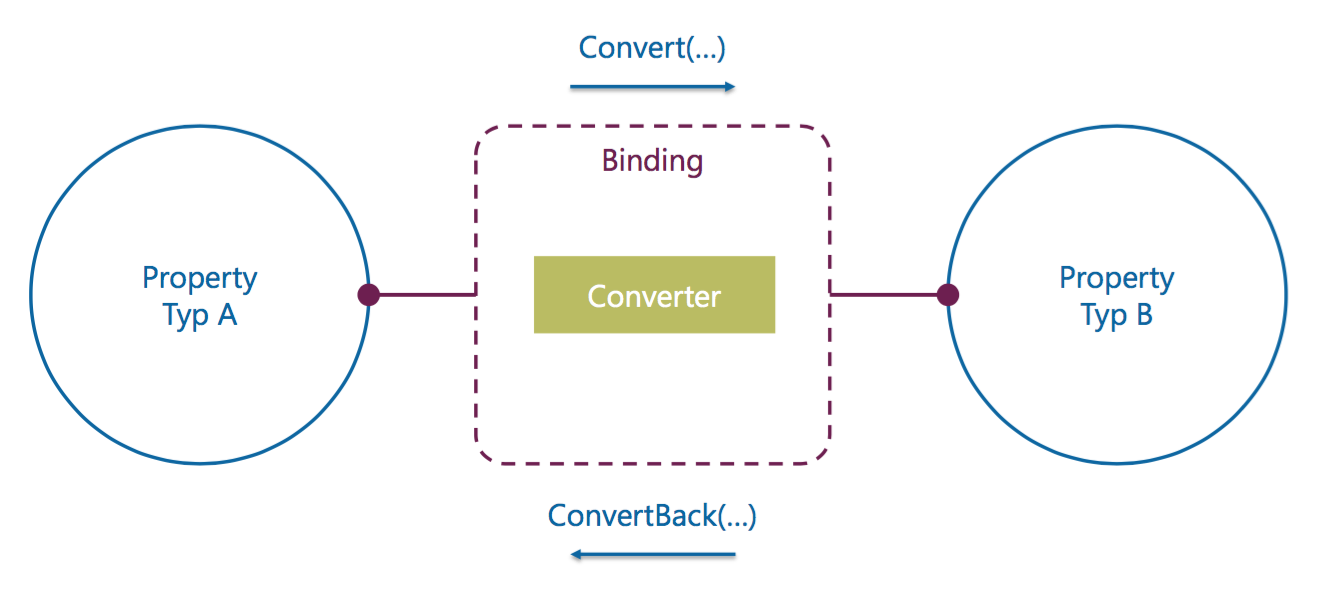
\includegraphics[scale=0.25]{IValueConverter.png}
\begin{lstlisting}[caption="Konvertiert bool oder Nullable in Visibility und zurück"]
public sealed class BooleanToVisibilityConverter: IValueConverter
{
    // value = bool oder nullable, targetType = Visibility
    public object Convert(object value, Type targetType, object parameter, CultureInfo culture)
    {
        return value is bool && (bool)value == true ? Visibility.Visible : Visibility.Collapsed;
    }
    // value = Visibility value, targetType = bool
    public object ConvertBack(object value, Type targetType, object parameter, CultureInfo culture)
    {
        return value as Visibility? == Visibility.Visible
    }
}
\end{lstlisting}
\paragraph{IMultiValueConverter} Das Interface dass alle MultiConverter implementieren müssen.
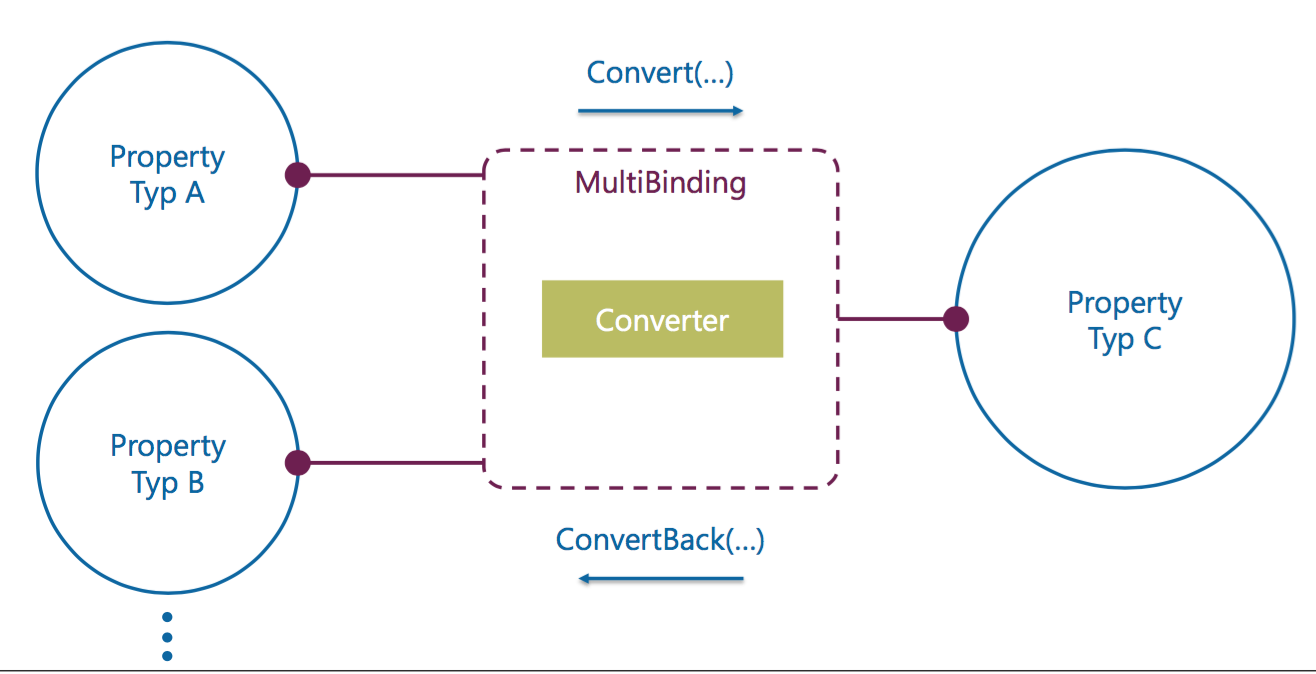
\includegraphics[scale=0.25]{IMultiValueConverter.png}
\begin{lstlisting}
public class RgbToColorConverter: IMultiValueConverter
{
    public object Convert(object[] values, Type targetType, object paramter, CultureInfo culture)
    {
        if (values == null)
            return DependencyProperties.Unsetvalue;
        if(values.Length != 3)
            throw new NotSupportedException("3 Values needed)";
        var r = (byte)System.Convert.ToInt32(values[0]);
        var g = (byte)System.Convert.ToInt32(values[1]);
        var b = (byte)System.Convert.ToInt32(values[2]);
        return Color.FromRgb(r,g,b);
    }
    public object[] ConvertBack(object value, Type[] targetType, object parameter, CultureInfo culture)
    {
        if(value == DependencyProperty.UnsetValue)
            return null;
        if(value is Color)
        {
            var color = (Color) value;
            var colors = new object[] {color.R, color.G, color.B};
            return colors;
        }
        return null;
    }
}
\end{lstlisting}
\paragraph{Value Converter anwenden} Um einen Converter anwenden zu können wird eine Instanz benötigt. Instanziierung:
\begin{lstlisting}[language=xml, caption="Instanzieren"]
<Window.Resources>
    <local:RgbToColorConverter x:Key="MyRgbToColorConverter" />
    <local:BestContrastingColorConverter x:Key="MyBestContrastingColorConverter" />
</Window.Resources>
\end{lstlisting}
Danach kann man den Converter wie gewohnt nutzen:
\begin{lstlisting}
<SolidColorBrush>
    <SolidColorBrush.Color>
        <MultiBinding Converter="{StaticResource MyRgbToColorConverter}">
            <Binding ElementName="ColorR" Path="Value"></Binding>
            <Binding ElementName="ColorG" Path="Value"></Binding>
            <Binding ElementName="ColorB" Path="Value"></Binding>
        </MultiBinding>
    </SolidColorBrush.Color>
</SolidColorBrush>
<SolidColorBrush Color="{Binding Path=Content, ElementName=ColorLabel,
    Converter={StaticResource MyBestContrastingColorConverter}, Mode=OneWay}" />
\end{lstlisting}
Wenn man eigene Value Converters implementiert wird der XAML Code kürzer und man hat eine Entkopplung von Wert und dessen Darstellungseigenschaften. Aber es ist aufwändig und teilweise nicht trivial.
\paragraph{Bindung auf eigene Objekte} Die sogenannten \textbf{DependencyProperties} ermöglichen ein Two-Way Binding und funktionieren mit Key-Value Dictionaries.Sie sind spezialisiert für die Vewendung in einem UI und somit nicht geeignet für Business Objects.
\begin{lstlisting}
public int MyProperty
{
  get {return (int(GetValue(MyPropertyPropert); }
  set { SetValue(MyPropertyProperty, value); }
}
public static readonly DependencyProperty MyPropertyProperty = 
    DependencyPropery.Register("MyProperty", 
            typeof(int), 
            typeoof(ownerclass), 
            new PropertyMetadata(0));
\end{lstlisting}
Mit dem \verb+INotifyPropertyChanged+ Interface können Properties einer Klasse überwacht werden. Das Interface schreibt das Event \verb+PropertyChanged+ vor, das implementiert werden muss. Der Event Handler übermittelt den Namen der geänderten Property.
\begin{lstlisting}
public class Person: INotifyPropertyChanged
{
    private string _firstName;
    public String FirstName
    {
        get {return _firstName; }
        set
        {
            if(value != _firstName)
            {
                _firstName = value;
                OnPropertyChanged(nameof(FirstName));
            }
        }
    }
    public event PropertyChangedeventHandler PropertyChanged;
    public void OnPropertyChanged(string name)
    {
        var handler = PropertyChanged;
        if (handler != null)
            handler(this, new PropertyChangedEventArgs(name));
    }
}
\end{lstlisting}
Dies kann auch mit einer Basisklasse gelöst werden, welche die Benachrichtigung implementiert.
\begin{lstlisting}
public abstract class BindableBase: INotifyPropertyChanged
{
    public event PropertyChangedEventHandler PropertyChanged;
    protected bool SetProperty<T>(ref T field, T value, string name = null)
    {
        if(Equals(field,value))
            return false;
        field=value;
        OnPropertyChanged(name);
        return true;
    }
    protected void OnPropertyChanged(string name = null)
    {
        PropertyChanged?.Invoke(this, new PropertyChangedEventArgs(name));
    }
}
public class Person: BindableBase
{
    private string _firstName;
    public string FirstName;
    {
        get { return _firstName; }
        set { SetProperty(ref _firstName, value, nameof(FirstName)); }
    }
}
\end{lstlisting}
\paragraph{Berechnete Properties} Möchte man Änderungen kommunizieren, sobald sich Quellwerte verändern, muss bei jedem Wechsel eine eigene Notification versendet werden. 
\begin{lstlisting}
protected bool SetProperty<T>(ref T storage, T value, string name, params string[] otherNames)
{
    if(Equals(storage, value))
        return false;
    storage = value;
    OnPropertyChanged(name);
    foreach(var n in otherNames)
        OnPropertyChanged(n);
    return true;
}
\end{lstlisting}
\paragraph{PropertyChanged.Fody} Fody ist ein Framwork, welches sich in den Kompilationsprozess einhängt und automatisch Properties überwacht. Damit Fody weiss welche Properties er überwachen muss, muss man es mit dem Attribut \verb+ImplementPropertyChanged+ markieren. 
\paragraph{ObservableCollection} Diese Klasse implementiert das INotifyCollectionChanged und INotifyPropertyChanged Interface. Diese Collection meldet Änderungen an sich automatisch, somit ist Event Handling auf neue Listeninhalte, bestimmte Positionen oder die gesamte Liste möglich.
\paragraph{ObjectDataProvider} Ermöglicht Verwendung einer beliebigen Datenquelle mit folgenden Zusatzmöglichkeiten. Es können Parameter an den Konstruktor übergeben werden (ConstructorParameters) oder es können Methoden inkl. Paramter gebunden werden (MethodParameters). Man kann damit beispielsweise Enums auf eine ComboBox binden.
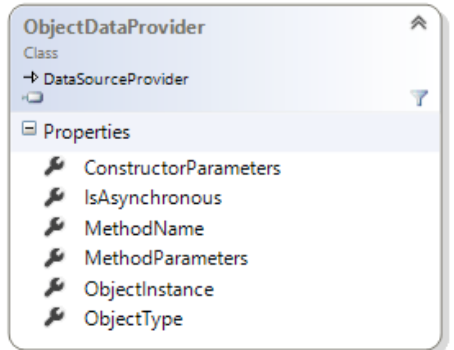
\includegraphics[scale=0.35]{ObjectDataProvider.png}
\begin{lstlisting}[language=xml]
<Window.Resources>
    <ObjectDataProvider x:Key="Alignments"
        MethodName="GetNames"
        ObjectType="{x:Type sys:Enum}">
    <ObjectDataProvider.MethodParameters>
        <x:Type TypeName="VerticalAlignment" />
    </ObjectDataProvider.MethodParameters>
    </ObjectDataProvider>
</Window.Resources>
<!-- Verwendung -->
<ComboBox ItemsSource="{Binding Source={StaticResource Alignments}}" />
\end{lstlisting}
\paragraph{DataBinding Debuggen} Man hat diverse Möglichkeiten die Abläufe hinter dem DataBinding sichtbar zu machen.
\begin{enumerate}
\item Direkt im Binding konfigurieren
\begin{lstlisting}[language=xml]
<!-- System.Diagnostics-Namespace - hinzufuegen -->
xmlns:diag="clr-namespace:System.Diagnostics;assembly=WindowsBase"
<!-- Binding Ausdruck um Setzten des TraceLevels erweitern -->
<TextBlock Text="{Binding ElementName=stack, Path=InvalidPath, diag:PresentationTraceSources.TraceLevel=High}" />
\end{lstlisting}
\item Dummy Converter schreiben
\begin{lstlisting}
public class DebugDummyConverter : IValueConverter
{
    public object Convert(object value, Type targetType, object parameter, CultureInfo culture)
    {
        return value;
    }
    public object ConvertBack(object value, Type targetType, object parameter, CultureInfo culture)
    {
        return value;
    }
}
\end{lstlisting}
\begin{lstlisting}[language=xml]
<Window.Resources> ... <local:DebugDummyConverter x:Key="MyDummy" /> ... </Window.Resources>
...
<TextBlock Text="{Binding ElementName=stack, Path=InvalidPath, Converter={StaticResource MyDummy}}" />
\end{lstlisting}
\item In VisualStudio DataBinding Debugging auf "{}All"{} setzten und im Output-Window nach \verb+Syste.Windows.Data+ suchen.
\end{enumerate}

\section{Benutzerinteraktion}
\paragraph{Routed Events} Events wandern vom Window den Visual Tree bis zum auslösenden Element. Routed Events besitzen meist ein Preview und ein normales Event. Das Preview Event wird ausgeführt, bevor es das Element erreicht, das normale Event, nachdem das Element das Event behandelt hat.
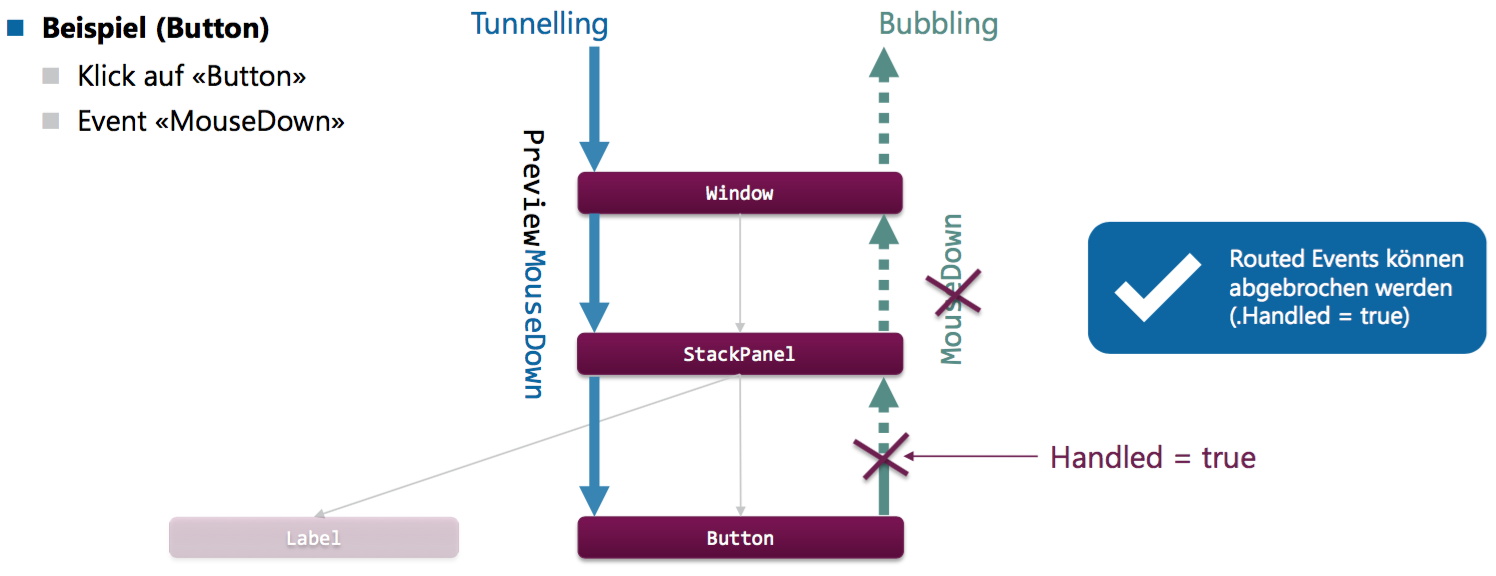
\includegraphics[scale=0.25]{RoutedEvent1.png}
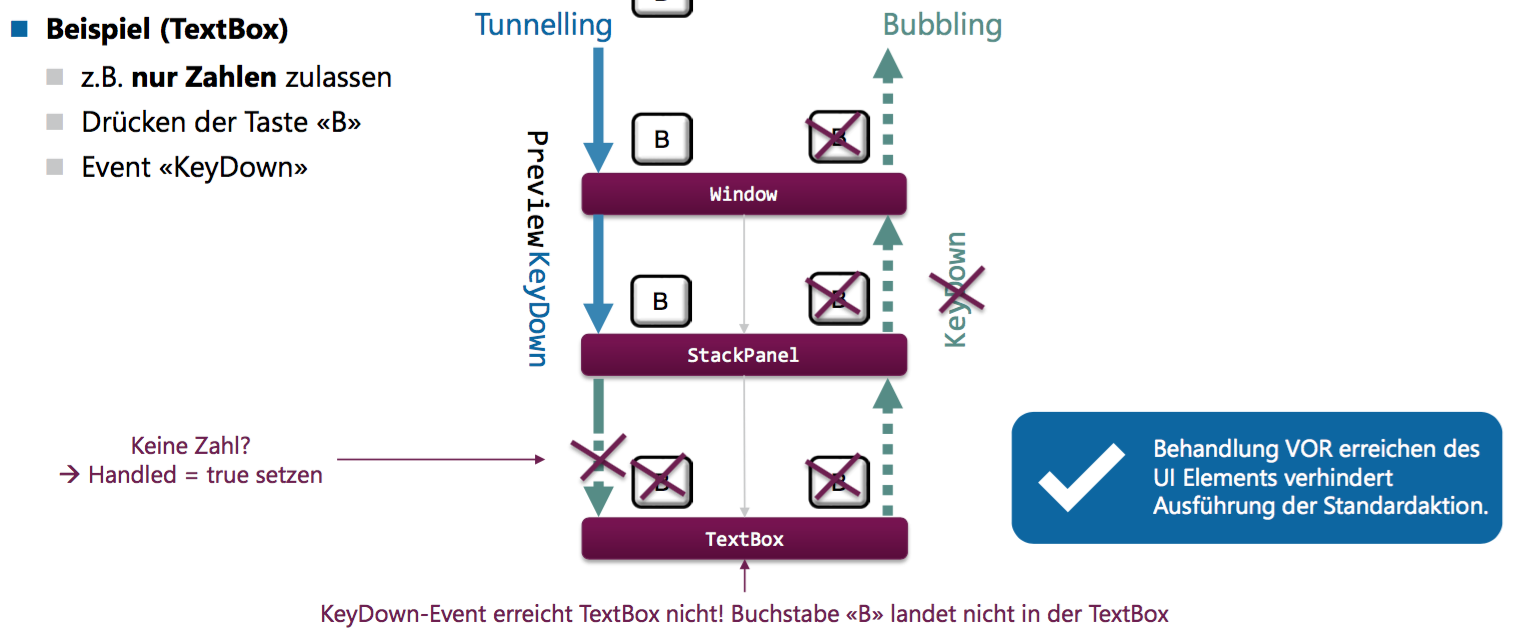
\includegraphics[scale=0.25]{RoutedEvent2.png}
Routed Events können mit \verb+Handeled = true+ unterbochen werden, sie werden dann nicht mehr weitergereicht. Man kann das Event direkt beim UI Element selbst behandeln.
\begin{lstlisting}[language=xml]
<Button Name="SaveButton"
    PreviewMouseDown="SaveButton_OnPreviewMouseDown"
    MouseDown="SaveButton_OnMouseDown">Save</Button>
\end{lstlisting}
Oder beim Parent Element
\begin{lstlisting}[language=xml]
<StackPanel PreviewMouseDown="StackPanel_OnPreviewMouseDown">
    ...
    <Button Name="SaveButton"
        PreviewMouseDown="SaveButton_OnPreviewMouseDown"
        MouseDown="SaveButton_OnMouseDown">Save</Button>
    ...
</StackPanel>
\end{lstlisting}
Eine andere Alternative wäre mit Attached Events.
\begin{lstlisting}[language=xml]
<StackPanel Button.Click="StackPanel_OnClick">
    ...
    <Button Name="SaveButton" Click="SaveButton_OnClick">Save</Button>
    ...
</StackPanel>
\end{lstlisting}
Beliebte Mouse Events:
\begin{tabular}{ll}
MouseDown & MouseEnter* \\
MouseLeave* & MouseLeftButtonDown \\
MouseLeftButtonUp & MouseMove \\
MouseRightButtonDown & MouseRightButtonUp \\
MouseUp & MouseWheel
\end{tabular}
Interessante Keyboard Events:
\begin{tabular}{ll}
KeyDown & KeyUp \\
TextInput & 
\end{tabular}
Interessante Touch-Events:
\begin{tabular}{ll}
TouchDown & TouchEnter* \\
TouchLeave* & TouchMove \\
TouchUp & 
\end{tabular}
* haben kein Preview Event.
\paragraph{RoutedEventArgs} RoutedEventArgs leiten von EventArgs ab. 
\begin{itemize}
\item \verb+Handled+: Boolean der aussagt, ob das Event behandelt wurde
\item \verb+OriginalSource+: Quell-Element (Hit-Testing) welches das Event ausgelöst hat
\item \verb+RoutedEvent+: Das RoutedEvent, welches mit diesem Objekt verknüpft ist
\item \verb+Source+: Element, welches das Event rapportiert hat
\end{itemize}
Die OriginalSource kann ein Kind-Element des Source-Elements sein, das per Hit-Testing als 1. Adressat des Events bestimmt wurde. Die Source ist das Element im Logical Tree, welches das Event rapportiert hat. Beispielsweise beim Subscribe auf MouseDown auf einem Button, wird das Event vom Button rapportiert (Source), wurde aber eigentlich vom Rahmen ausgelöst (OriginalSource).
\paragraph{Ableitende Klasse von RoutedEventArgs} Es gibt für verschiedene Input-Geräte Ableitungen von RoutedEventArgs. Auswahl von \verb+MouseEventArgs+:
\begin{itemize}
\item \textbf{LeftButton}: Zustand der linken Maustaste (Pressed/Released)
\item \textbf{MiddleButton}
\item \textbf{RightButton}
\item \textbf{Delta}: Mausradbewegung (-120/120)
\end{itemize}
Auswahl von \verb+KeyEventArgs+:
\begin{itemize}
\item \textbf{Key}: Taste (Enum)
\item \textbf{IsDown}
\item \textbf{IsUp}
\item \textbf{IsRepeat}
\item \textbf{SystemKey}: Die zusätzliche Taste, falls ALT-Taste gedrückt wurde. Key steht in \verb+Key.System+
\end{itemize}
\subsection{Drag \& Drop}
Drag \& Drop besteht aus 3 Phasen:
\begin{enumerate}
\item \textbf{Maustaste wird gedrückt:} Nach überschreiten einer Mindestdistanz wird die Aktion gestartet
\item \textbf{Während des Ziehens:} Steuerelemente unterhalb des Zeigers müssen melden, ob sie als Ziel infrage kommen
\item \textbf{Fallenlassen:} Steuerelement unterhalb des Mauszeigers muss eine Aktion mit dem bewegten Objekt durchführen
\end{enumerate}
Beispiel:
\begin{lstlisting}
public ObservableCollection<UserInfo> AvailableUsers { get; set; }
public ObservableCollection<UserInfo> SelectedUsers { get; set; }
public MainWindow()
{
    // Listen initialisieren und fuellen
    InitializeComponent();
    DataContext = this;
}
\end{lstlisting}
\paragraph{Phase 1} Maustaste wird gedrückt
\begin{lstlisting}[language=xml]
<ListBox Name="AvailableListBox" ItemsSource="{Binding AvailableUsers}"
    ItemTemplate="{StaticResource UserInfoTemplate}"
    PreviewMouseLeftButtonDown="AvailableListBox_ OnPreviewMouseLeftButtonDown"
    PreviewMouseLeftButtonUp="AvailableListBox_ OnPreviewMouseLeftButtonUp"
    MouseMove="AvailableListBox_OnMouseMove" />
\end{lstlisting}
\begin{lstlisting}
private Point? dragStartPosition = null;
private void AvailableListBox_ OnPreviewMouseLeftButtonUp(object sender, MouseButtonEventArgs e)
{
    dragStartPosition = null;
}
private void AvailableListBox_ OnPreviewMouseLeftButtonDown(object sender, MouseButtonEventArgs e)
{
    dragStartPosition = e.GetPosition(this);
}
private bool IsMovementFarEnough(Point origPos, Point curPos)
{
    var minDistX = SystemParameters.MinimumVerticalDragDistance;
    var minDistY = SystemParameters.MinimumHorizontalDragDistance;
    return (Math.Abs(curPos.X - origPos.X) >= minDistX || Math.Abs(curPos.Y - origPos.Y) >= minDistY);
}
private void AvailableListBox_OnMouseMove(object sender, MouseEventArgs e)
{
    // gar nicht starten, wenn nicht (innerhalb Liste) geklickt
    if (dragStartPosition == null)
        return;
    // aktuelle Position holen und pruefen, ob die Maus genug
    // bewegt wurde, um die Bewegung als Drag zu interpretieren
    var position = e.GetPosition(this);
    if (!IsMovementFarEnough(dragStartPosition.Value, position))
        return;
    // Alles ok, drag kann starten
    dragStartPosition = null;
    StartDrag(AvailableListBox.SelectedItem as UserInfo);
}
private void StartDrag<T>(T obj)
{
    // Bereich definieren, auf dem der Drag-Vorgang gueltig ist
    var dragScope = this.Content as FrameworkElement;
    // Container fuer Nutzdaten (hier String)
    var dragData = new DataObject(typeof(T), obj);
    // Drag-Vorgang starten
    DragDrop.DoDragDrop(dragScope, dragData, DragDropEffects.Move);
}
\end{lstlisting}
Die \verb+DragDrop.DoDragDrop+ Methode blockiert die weitere Code-Ausführun bis die Operation beendet ist.
\paragraph{Phase 2} Maus wird gezogen
\begin{lstlisting}[language=xml]
<ListBox Name="SelectedListBox" ItemsSource="{Binding SelectedUsers}"
    ItemTemplate="{StaticResource UserInfoTemplate}"
    AllowDrop="True"
    DragOver="SelectedListBox_OnDragOver"
    Drop="SelectedListBox_OnDrop" />
\end{lstlisting}
\begin{lstlisting}
private void SelectedListBox_OnDragOver(object sender, DragEventArgs e)
{
    // Objekt auspacken
    var data = e.Data.GetData(typeof(UserInfo)) as UserInfo;
    // falls Objekt verfuegbar, dann kopieren, sonst keine Operation
    e.Effects = data != null ? DragDropEffects.Copy : DragDropEffects.None;
}
\end{lstlisting}
\paragraph{Phase 3} Objekt wird fallengelassen
\begin{lstlisting}[language=xml]
<ListBox Name="SelectedListBox" ItemsSource="{Binding SelectedUsers}"
    ItemTemplate="{StaticResource UserInfoTemplate}"
    AllowDrop="True"
    DragOver="SelectedListBox_OnDragOver"
    Drop="SelectedListBox_OnDrop" />
\end{lstlisting}
\begin{lstlisting}
private void SelectedListBox_OnDrop(object sender, DragEventArgs e)
{
    // Objekt auspacken
    var user = e.Data.GetData(typeof(UserInfo)) as UserInfo;
    // Dank Data Binding reicht es nun, das UserInfo Objekt
    // der ObservableCollection hinzuzufuegen:
    SelectedUsers.Add(user);
}
\end{lstlisting}
\paragraph{Drag \& Drop Events}
\begin{itemize}
\item \textbf{DragEnter:} Tritt auf, wenn dieses Element während einer Drag-Operation als Drag Target fungieren würde (Hit-Testing)
\item \textbf{DragLeave:} Tritt auf, wenn dieses Element während einer Drag-Operation verlassen wird
\item \textbf{DragOver:} Tritt auf, wenn diesem Element eine Drag-Operation stattfindet
\item \textbf{Drop:} Tritt auf, wenn das Objekt der Drag-Operation auf dieses Element fallengelassen wird
\item \textbf{GiveFeedback:} Gibt der Quelle der Drag-Operation eine Chance, visuelles Feedback zu geben
\end{itemize}
\section{Hintergrund-Operationen}
Lange Dauernde Operationen sollten nicht im UI-Thread ausgeführt werden, sonden in ein eigenen Thread ausgelagert werden, sodass das UI nicht einfriert. Um den Benutzer zu informieren, dass irgendwas "{}arbeitet"{} sollte man folgendermassen vorgehen:
\begin{enumerate}
\item Visuelles Feedback geben (Spinner, Overlay, Popup), wenn nötig
\item Starten eines Background-Threads als Reaktion auf ein Event, Kontrolle an UI Thread zurückgeben
\item Bei Thread-Ende aus dem Background-Thread den UI-Thread benachrichtigen
\end{enumerate}
\paragraph{Visuelles Feedback} Das visuelle Feedback umfasst auch, dass der Benutzer dieselbe Operation nicht aus versehen zweimal ausführt. Dies verhindert man, indem man beispielsweise den Button deaktiviert etc. Um dem Benutzer mittzuteilen, dass etwas läuft, kann man beispielsweise ein Spinner auf den Button legen (realisierbar durch Grid innerhalb des Buttons). 
%TODO: Eventuell noch XAML Beispiel
\paragraph{Starten eines Background Threads} Dazu verwendet man am besten die Task Paralell Library. 
\begin{lstlisting}
Task.Run(() => {
    //Background operation
});
\end{lstlisting}
\paragraph{UI-Thread benachrichtigen} Mit der TPL kann man einen Dispatcher verwenden, um Code im UI-Thread auszuführen.
\begin{lstlisting}
Task.Run(() => {
    //Background operation
    Dispatcher.Invoke(() => {
        // UI interaktion
    });
});
\end{lstlisting}
Falls Dispatcher nicht aus Code-Behind aufgerufen wird (Dispatcher ist eine Property der UI-Elemente wie Window, muss man stattdessen \verb+System.Windows.Threading.Dispatcher.CurrentDispatcher+ verwenden.
\end{multicols*}
\end{document}
